\documentclass{mini}

\usepackage[utf8]{inputenc}
\usepackage{color}
\usepackage{xcolor}
\usepackage{colortbl}
\usepackage{tikz}
\usepackage{tikz-qtree}
\usepackage{caption}
\usepackage{subcaption}
\usepackage{multirow}
\usepackage{tabularx}
\usepackage{lscape}
\usepackage{verbatim}
\usepackage{algorithm}
\usepackage{algorithmic}
%\usepackage[noend]{algpseudocode}
\usepackage{caption}


\makeatletter
\renewcommand{\ALG@name}{Algorytm}
\makeatother

\setlength{\extrarowheight}{3pt}
\usetikzlibrary{calc, shapes, backgrounds, arrows, positioning, calc}

\definecolor{mojkolor}{rgb}{0.99, 1, 0.99}
\newenvironment{dow}{\textbf{\textit{Dowód}}}{\begin{flushright} $\blacksquare$ \end{flushright}}
\newcommand{\argmin}{\arg\!\min}
\newcommand{\argmax}{\arg\!\max}

\newlength\myindent
\setlength\myindent{2em}
\newcommand\bindent{%
  \begingroup
  \setlength{\itemindent}{\myindent}
  \addtolength{\algorithmicindent}{\myindent}
}
\newcommand\eindent{\endgroup}

%------------------------------------------------------------------------------%
\title{Statystyczne metody regresji porządkowej}
\titleaux{Statistical methods for ordinal regression}
\author{Marta Sommer}
\tytsupervisor{prof. nzw. dr hab.}
\supervisor{Przemysław Grzegorzewski}
\type{magisters}
\discipline{matematyka}
\monthyear{grudzień 2015}
\date{\today}
\album{237503}
%------------------------------------------------------------------------------%

\begin{document}

\maketitle
\tableofcontents

\chapter*{Wstęp}

Uczenie maszynowe jest bardzo szybko rozwijającym się zagadnieniem z pogranicza matematyki i informatyki. Główną przyczyną tego zjawiska jest jego szeroka gama zastosowań. Już nawet prosta regresja i klasyfikacja pomagają w odkrywaniu pewnych zależności oraz pozwalają prognozować różne wielkości. Z uczeniem maszynowym bardzo często -- choć nie zawsze świadomie -- spotykamy się w życiu codziennym np. korzystając z systemów rekomendacyjnych, czy używając wyszukiwarki internetowej. To właśnie z tych praktycznych zastosowań wynikła potrzeba stworzenia tzw. regresji porządkowej (ang. \textit{ordinal regression}). Zanim poznamy formalną definicję tego zagadnienia i zagłębimy się w temat, prześledźmy poniższy przykład, by wyrobić sobie pewną intuicję, czym właściwie jest regresja porządkowa.  

Wyobraźmy sobie sytuację, że chcielibyśmy przewidzieć, w jakim stopniu potencjalnemu klientowi spodoba się sprzedawany przez nas produkt. Mając taką wiedzę, moglibyśmy bowiem przewidywać, co opłaca się mu polecić bądź zareklamować. Chcąc uprościć analizę, skupimy się na następujących możliwych odpowiedziach klienta: \textit{zdecydowanie mi się nie podoba}, \textit{nie podoba mi się}, \textit{nie mam zdania}, \textit{podoba mi się}, \textit{zdecydowanie mi się podoba}. Z jednej strony mamy do dyspozycji pewne cechy danego klienta. Przykładowo, mogą to być jego wiek, płeć czy wykształcenie. Nie zawsze jednak potrafimy uzyskać takie dane -- szczególnie, gdy~nie mamy bezpośredniego kontaktu z klientem, bo prowadzimy np. sklep internetowy. Wtedy jako wektor cech możemy przyjąć np. jego historię zakupów na naszej stronie. Z drugiej strony mamy też pewną grupę klientów, o których wiemy, co myślą o danym produkcie (bo np. zapytaliśmy ich o to wprost lub za pomocą ankiety). Metoda działania powinna być więc następująca. Najpierw -- na danych historycznych -- dopasowujemy pewien model, a następnie, gdy przychodzi do nas klient o konkretnych cechach, używając wcześniej skonstruowanego modelu, dostajemy odpowiedź, czy produkt mu się spodoba czy nie. 

Analizę powyższego problemu można przeprowadzić na kilka różnych sposobów. Najbardziej naturalnym wydawałoby się zastosowanie klasyfikacji wieloetykietowej (tzn. takiej, gdzie odpowiedź jest nominalna i ma więcej niż dwa poziomy). Tracimy wtedy jednak istotną informację o tym, że odpowiedzi tworzą pewien naturalny porządek. Chcąc niejako wziąć to pod~uwagę, można potraktować nasz problem jak zwykłą regresję, zamieniając zmienną odpowiedzi w pewną zmienną ciągłą (np. \textit{zdecydowanie mi się nie podoba} odpowiadałoby cyfrze $1$, a \textit{zdecydowanie mi się podoba} cyfrze $5$) i to ją modelować, a następnie z powrotem dyskretyzować. Pojawia się tu jednak problem, jak optymalnie zrobić taką transformację, uwzględniając chociażby fakt, że nasze odpowiedzi niekoniecznie są od siebie jednakowo odległe (tzn. np. różnica między \textit{nie podoba mi się} a \textit{nie mam zdania} wcale mnie musi być taka sama, jak~między \textit{podoba mi się} a \textit{zdecydowanie mi się podoba}). Podstawowe zagadnienia uczenia maszynowego nie znajdują tu zatem zastosowania i stąd wynikło zapotrzebowanie rozwinięcia problemu regresji porządkowej. 

Powyższy przykład wyrobił nam pewną intuicję co do tego, czym jest regresja porządkowa. Krótko określić można by ją było jako problem klasyfikacji wieloetykietowej, w którym zmienna odpowiedzi tworzy pewien naturalny porządek. Formalne sformułowanie problemu przedstawię na początku rozdziału pierwszego.

Celem mojej pracy jest teoretyczne i praktyczne omówienie regresji porządkowej. Praca ma zatem następującą strukturę. Rozdział pierwszy poświęcony został zebraniu, opisaniu i usystematyzowaniu dostępnych w literaturze metod modelowania tego zagadnienia. Pokazane są w nim również wady i zalety różnych podejść do tematu oraz różnice między nimi. W~rozdziale drugim opisane zostały metody diagnostyki modelu oraz ich mocne i słabe strony. W~ostatnim rozdziale, który -- w przeciwieństwie do bardzo teoretycznych pierwszych dwóch -- opiera się na danych rzeczywistych, porównamy metody modelowania regresji porządkowej oraz ocenimy jakość współczynników diagnostycznych.       


%Możemy wyróżnić dwa główne nurty w regresji porządkowej:
%\begin{itemize}
%	\item prognoza konkretnej obserwacji (nacisk kładziony jest tu na wyznaczenie konkretnego $\textbf{y}$ dla %konkretnego $\textbf{x}$ np. czy potencjalnemu klientowi spodoba się dany produkt),
%	\item uszeregowanie kilku obserwacji (celem nie jest poznanie estymacji konkretnej zmiennej odpowiedzi, ale takie %uszeregowanie kilku rekordów, by te najbardziej preferowane znalazły się na samej górze, a te najmniej na samym dole %np. w jakiej kolejności powinny wyświetlić się znalezione strony w wyszukiwarce). 
%\end{itemize}
%
%W mojej pracy zajmować się będę przede wszystkim pierwszym punktem, lecz nakreślę też kilka podejść dotyczących %drugiego. 


\chapter{Opis teoretyczny dostępnych metod}


\section{Postawienie problemu i podstawowe oznaczenia}

Na wejściu dany mamy zbiór $\mathcal{D} = (\mathbf{x}^{(i)}, y^{(i)})_{i=1}^n$, składający się z $n$ par $(\mathbf{x}, y)$, gdzie:
\begin{itemize}
\item $\mathbf{x}^{(i)}$ jest $K$--wymiarowym wektorem cech (częstym założeniem będzie, że $\mathbf{x}^{(i)}\in \mathbb{R}^K$),  
\item $y^{(i)}$ jest liczbą symbolizującą kategorię, do której przyporządkowana została $i$--ta obserwacja, tzn. $y^{(i)}\in\mathcal{Y}$, gdzie $\mathcal{Y} = \lbrace 1,\ldots ,r \rbrace$ jest zbiorem uporządkowanym według pewnego porządku ,,$\prec$''. 
\end{itemize}
Naszym celem będzie stworzenie modelu, który pozwoli na wybranie najlepszej (nieznanej) kategorii $y_{\ast}\in\mathcal{Y}$ dla nowej obserwacji o zadanym wektorze cech $\mathbf{x}_{\ast}$. 

W tym rozdziale opracujemy kilka rozwiązań, które pozwolą nam się z tym problemem uporać.

\section{Model proporcjonalnych szans}

Najbardziej rozpowszechnionym sposobem modelowania regresji porządkowej jest model proporcjonalnych szans (ang. \textit{proportional odds model}), patrz \cite{pom}. Jest to jedna z metod uogólnionych modeli liniowych, bardzo silnie opierająca się na regresji logistycznej. Interesują nas prawdopodobieństwa: 
$$
\Pi_j(\mathbf{x}):=\mathbb{P}(y=j\hspace{1mm}|\hspace{1mm}\mathbf{x}),\quad \textrm{dla}\hspace{3mm} j=1,\ldots,r.
$$
Idea tej metody polega nie na bezpośrednim szukaniu prawdopodobieństw $\Pi_j(\mathbf{x})$, lecz na wcześniejszym modelowaniu tzw. prawdopodobieństw skumulowanych:
$$
\mathbb{P}(y\leq j \hspace{1mm}|\hspace{1mm} \mathbf{x})=\Pi_1(\mathbf{x})+\ldots+\Pi_j(\mathbf{x}),\quad \textrm{dla}\hspace{3mm} j=1,\ldots,r-1.
$$
Następnie rozważa się poniższy model logitowy:
$$
\log\dfrac{\mathbb{P}(y\leq j \hspace{1mm}|\hspace{1mm} \mathbf{x})}{1 - \mathbb{P}(Y\leq j \hspace{1mm}|\hspace{1mm} \mathbf{x})} = \alpha_j+\mathbf{\beta}^T\mathbf{x},\quad \textrm{dla}\hspace{3mm} j=1,\ldots,r-1,
$$
gdzie $\alpha_j\in \mathbb{R}$ i $\mathbf{\beta}\in \mathbb{R}^K$ są parametrami modelu. Należy zauważyć, że parametr $\beta$ jest stały dla każdego $j=1, \ldots, r-1$.

Współczynniki modelu -- jak w przypadku regresji logistycznej -- wyliczamy metodą Raphsona-Newtona, a skumulowane prawdopodobieństwa -- po prostym przeliczeniu -- dostaniemy ze~wzoru:
$$
\mathbb{P}(y\leq j \hspace{1mm}|\hspace{1mm} \mathbf{x})=\dfrac{e^{\alpha_j+\mathbf{\beta}^T\mathbf{x}}}{1+e^{\alpha_j+\mathbf{\beta}^T\mathbf{x}}},\quad \textrm{dla}\hspace{3mm} j=1,\ldots,r-1.
$$ 
Szukane prawdopodobieństwa $\Pi_j(\mathbf{x})$ otrzymamy w poniższy sposób:
\begin{eqnarray*}
\Pi_1(\mathbf{x}) &=& \mathbb{P}(Y\leq 1 \hspace{1mm}|\hspace{1mm}\mathbf{x}),\\
&\vdots&\\
\Pi_i(\mathbf{x}) &=& \mathbb{P}(Y\leq i \hspace{1mm}|\hspace{1mm} \mathbf{x}) - \mathbb{P}(Y\leq i-1 \hspace{1mm}|\hspace{1mm} \mathbf{x}),\\
&\vdots&\\
\Pi_r(\mathbf{x}) &=& 1 - \mathbb{P}(Y\leq r-1 \hspace{1mm}|\hspace{1mm} \mathbf{x}).
\end{eqnarray*}

Dla nowej obserwacji $\mathbf{x}_{\ast}$ wybieramy, oczywiście, tę klasę $y_{\ast}$, która maksymalizuje prawdopodobieństwa $\Pi_j(\mathbf{x}_{\ast})$.

\section{Wektory maszyn podpierających (SVM)}

Wektory maszyn podpierających (ang. \textit{Support Vector Machine}) to bardzo znana i powszechnie stosowana metoda klasyfikacji (patrz \cite{koronacki}). W dużym uproszczeniu, polega ona na konstrukcji dwóch równoległych i maksymalnie oddalonych od siebie hiperpłaszczyzn rozdzielających klasy. By móc obsługiwać przypadki, w których brak liniowej separowalności, wprowadza się dodatkowo karę za nieidealne rozdzielenie klas. W przypadku dwuklasowym (patrz Rys.\ref{svm1}) budowa modelu sprowadza się do rozwiązania następującego problemu optymalizacyjnego:
$$
\min_{\mathbf{w}, b}\left\lbrace\dfrac{1}{2}||\textbf{w}||^2+C\sum_{i=1}^{n}\xi_i\right\rbrace,
$$
przy ograniczeniach:
$$
\begin{cases}
\mathbf{x}^T_{1i}\textbf{w}+b &\geq +1-\xi_i, \hspace{6mm} \text{dla}\hspace{3mm}i=1\ldots n_1 \\
\mathbf{x}^T_{2i}\textbf{w}+b &\leq -1+\xi_i, \hspace{6mm} \text{dla}\hspace{3mm}i=1\ldots n_2
\end{cases}
$$    
gdzie $\mathbf{w}\in\mathbb{R}^K$, $b\in\mathbb{R}$ i $C\in\mathbb{R}$ są parametrami modelu, $\xi_i\geq 0$ dla $i=1\ldots n$ są karą mierzoną dla każdej obserwacji przy ustalonej hiperpłaszczyźnie, $\mathbf{x}_{1i}$ oznacza wektor cech obserwacji należących do klasy pierwszej, a $\mathbf{x}_{2i}$ wektor cech obserwacji należących do klasy drugiej, zaś $n_1$ i $n_2$ to liczności tych klas. 

\begin{figure}[]
  \begin{subfigure}[]{\textwidth}
    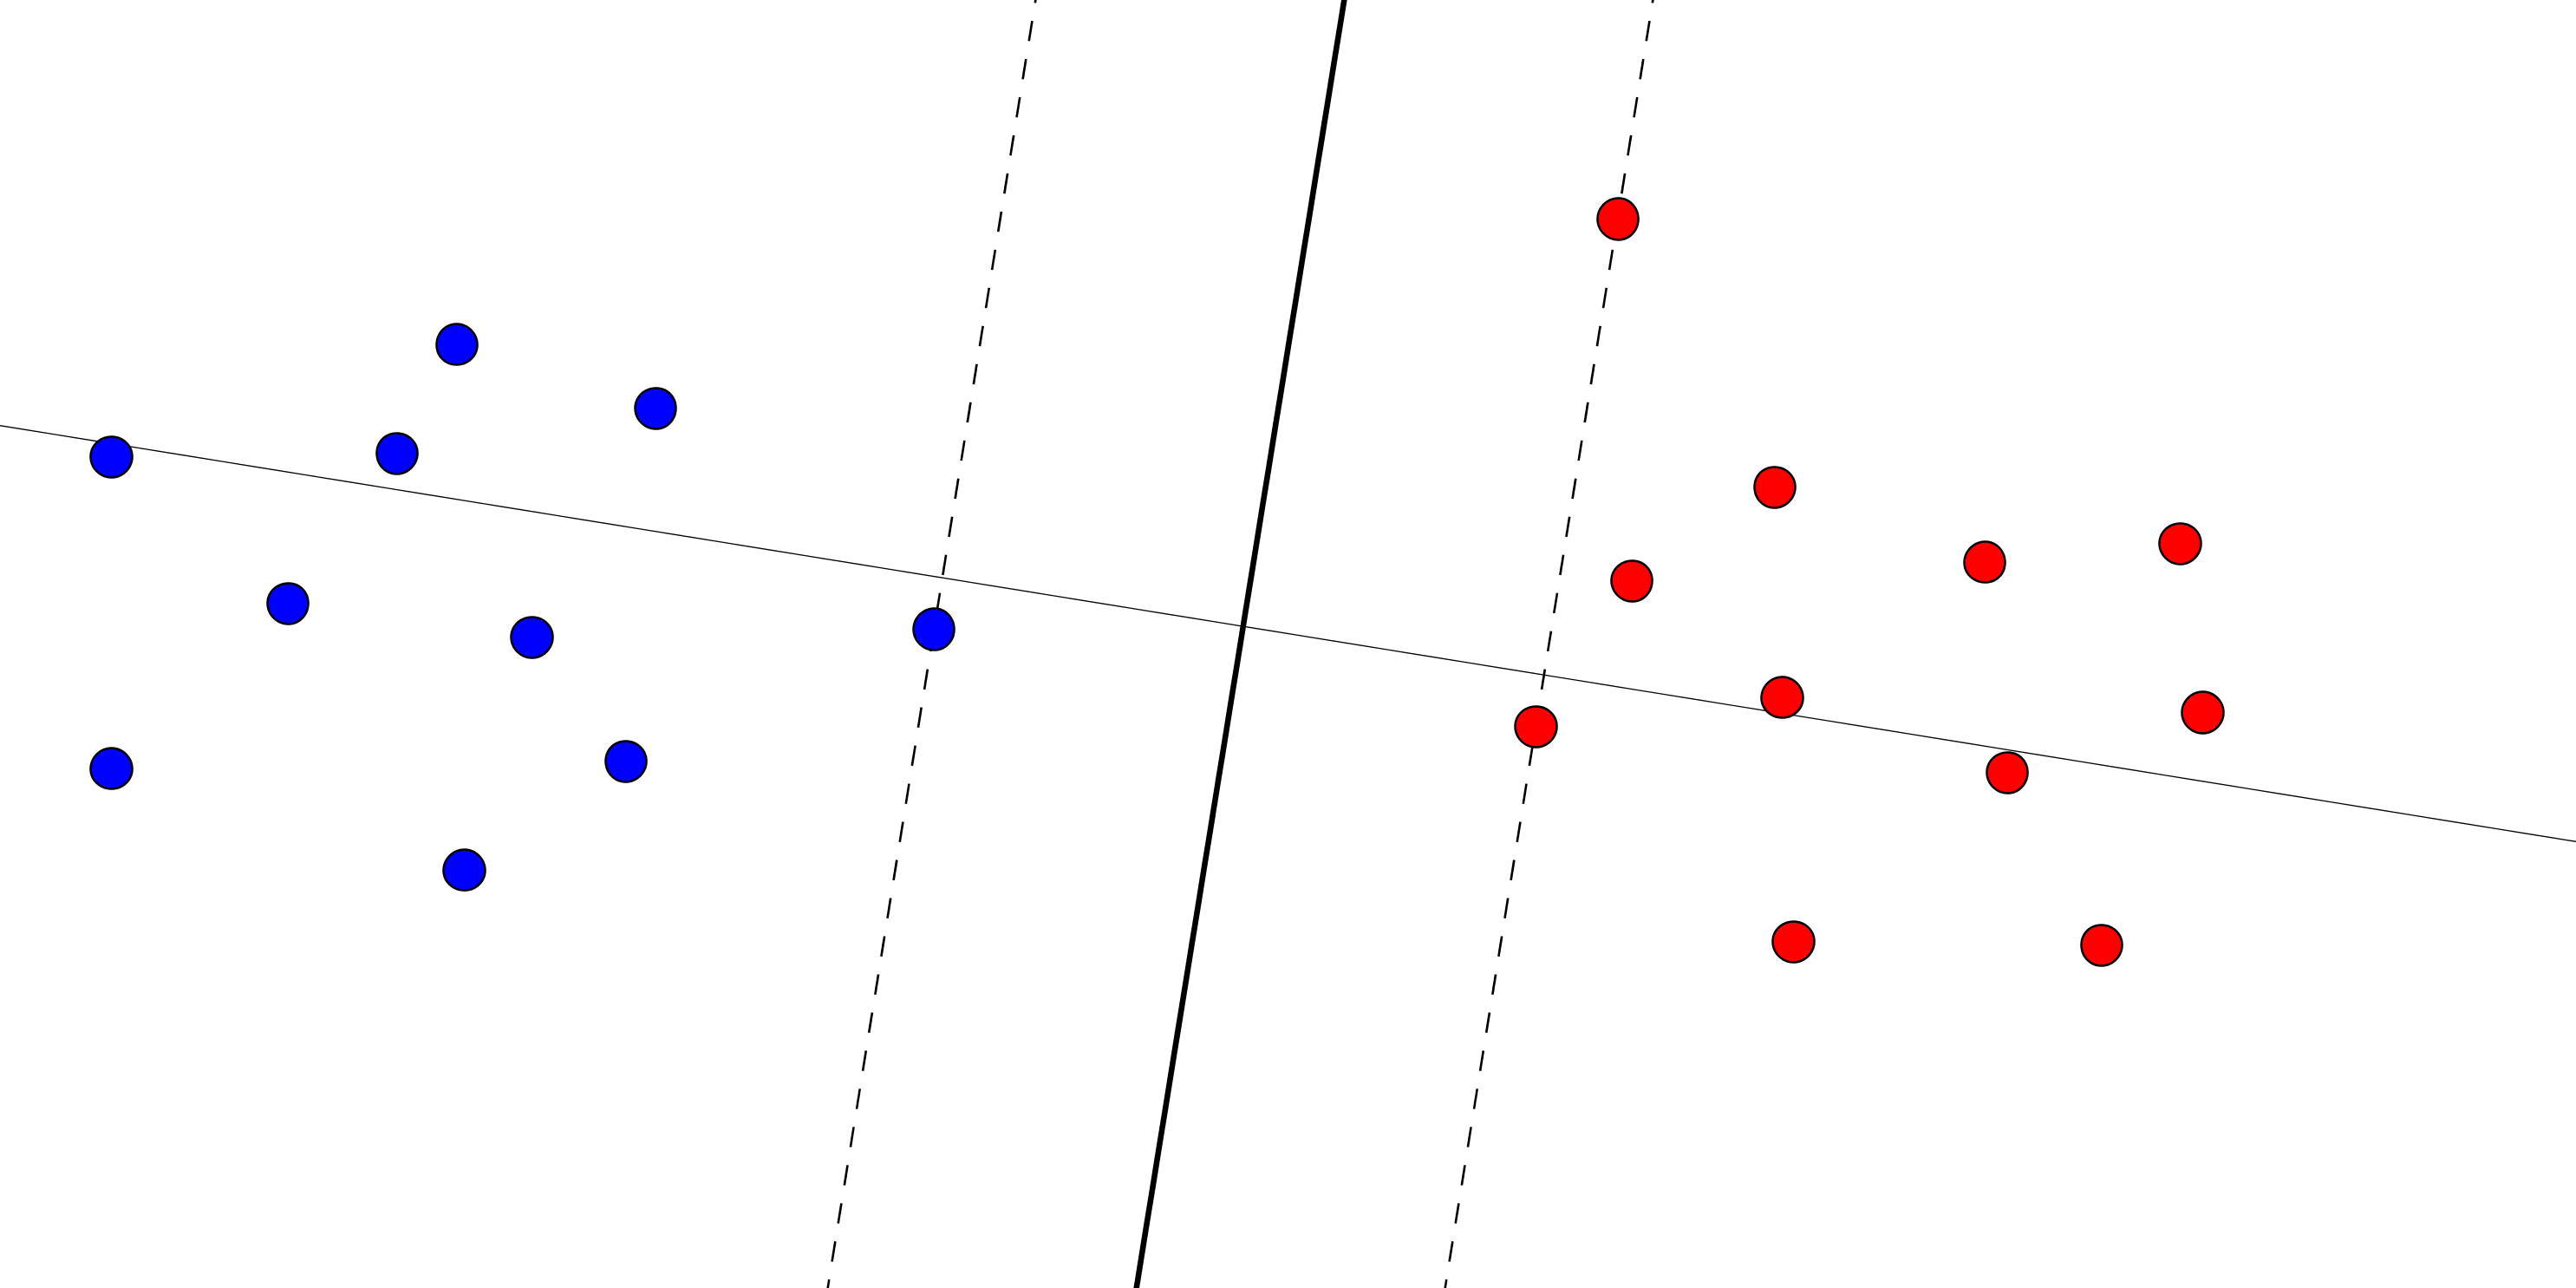
\includegraphics[width=\textwidth]{graphics/svm1.png}
    \caption{Przypadek separowalny.}
  \end{subfigure}
  %\hfill
  \begin{subfigure}[]{\textwidth}
    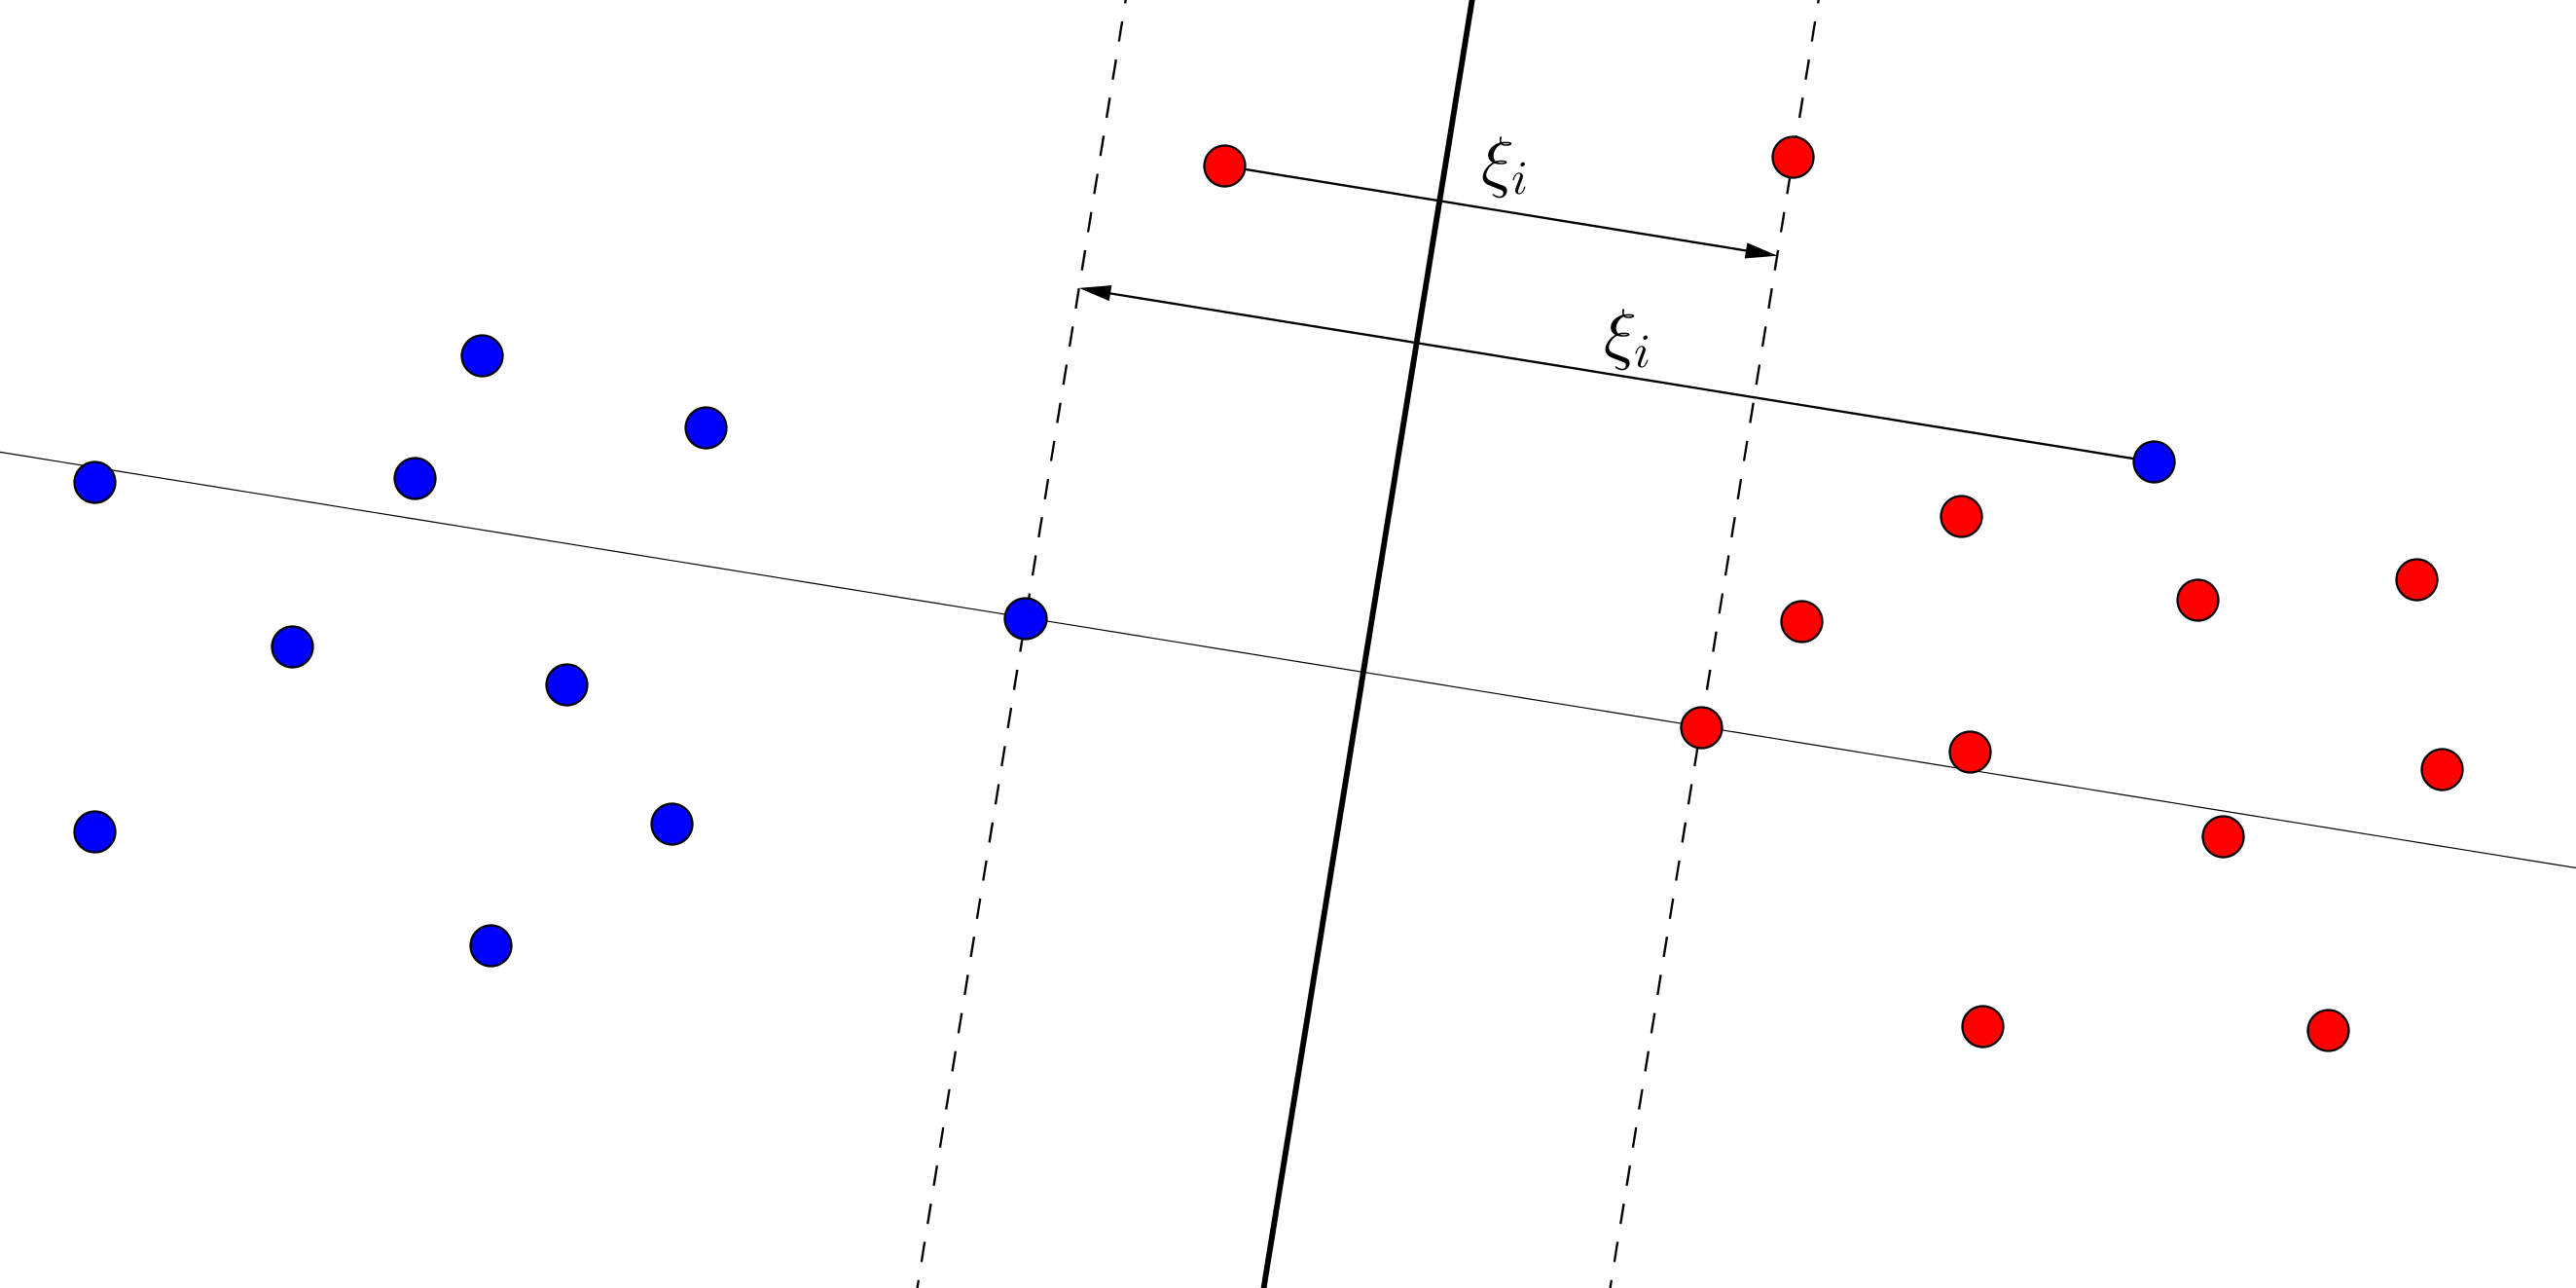
\includegraphics[width=\textwidth]{graphics/svm1eps.png}
    \caption{Przypadek nieseparowalny.}
  \end{subfigure}
  \caption{Przykładowe rozdzielenie klas metodą SVM. W przypadku nieseparowalnym dokładamy karę, będącą odległością źle zaklasyfikowanej obserwacji od odpowiedniego marginesu.}
  \label{svm1}
\end{figure}

Tak to wygląda w przypadku klasyfikacji dwuklasowej. Przyjrzyjmy się teraz, jak w łatwy sposób można zaadaptować powyższą metodę do rozważanej przez nas regresji porządkowej.

\begin{figure}[h]
\begin{center}
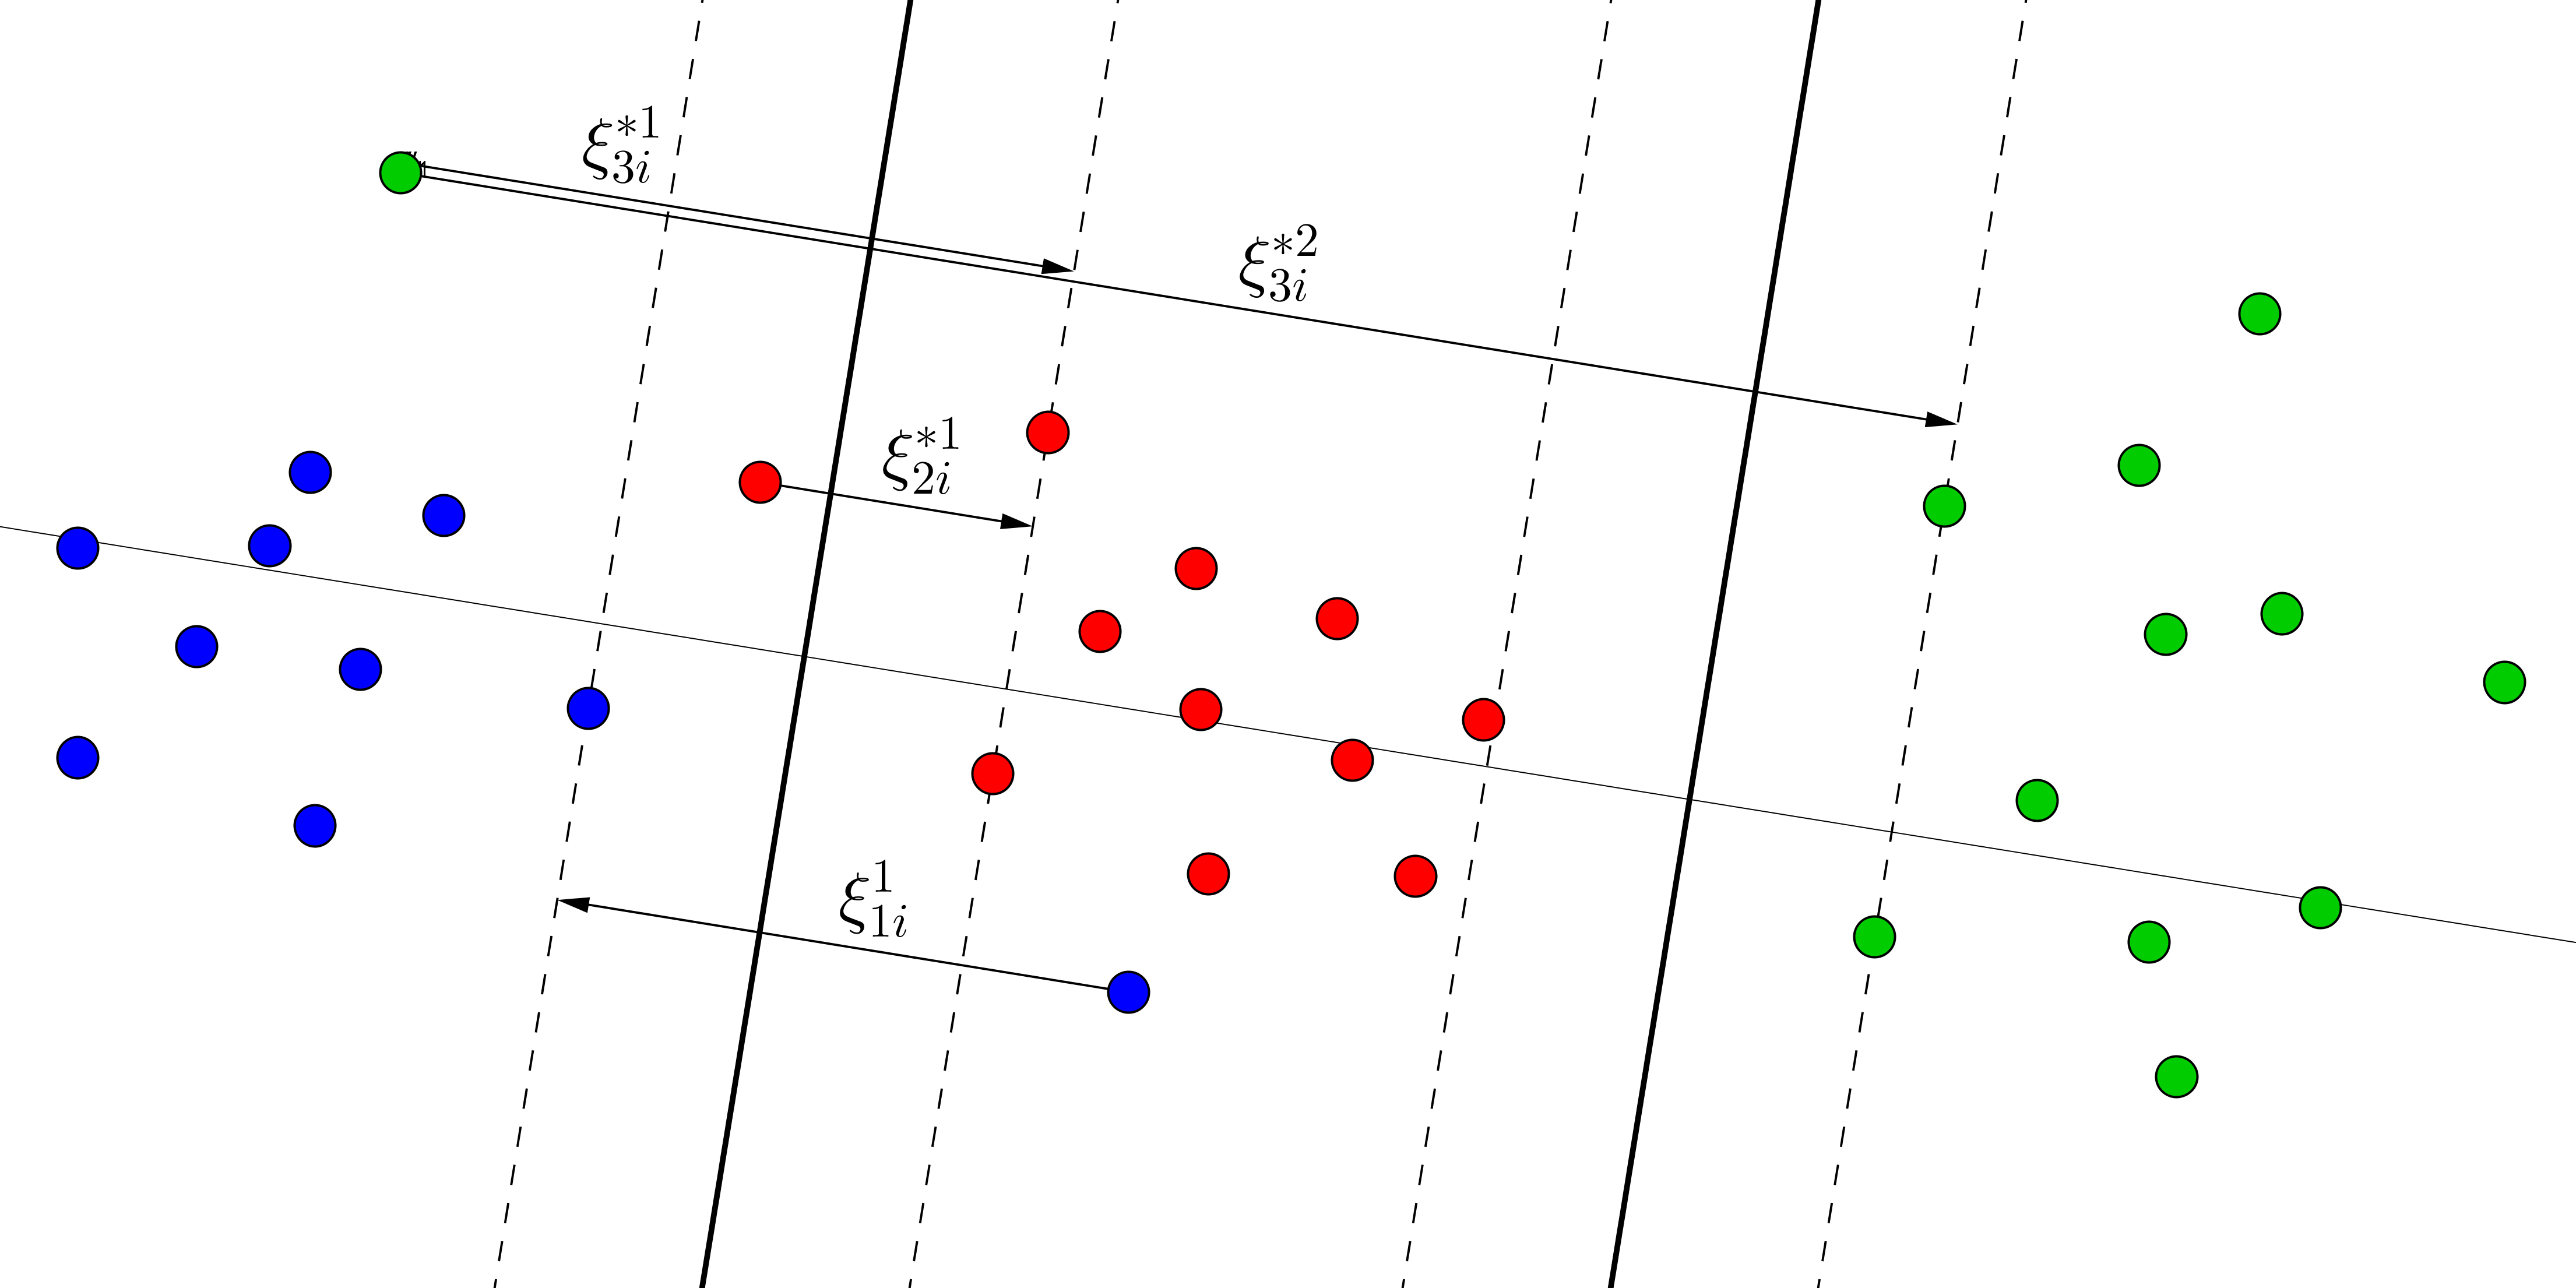
\includegraphics[width=\textwidth]{graphics/svm3.png}
\end{center}
\caption{Przykładowa klasyfikacja metodą SVM.}
\label{svm}
\end{figure}

Tym razem, powołując się na \cite{pom} i \cite{svm}, będziemy rozwiązywać następujący problem optymalizacyjny:
$$
\min_{\textbf{w}, b_1, \ldots, b_{r-1}}\left\lbrace \dfrac{1}{2}||\textbf{w}||^2+C\sum_{j=1}^{r-1}\left( \sum_{k=1}^{j}\sum_{i=1}^{n_k}\xi_{ki}^j+\sum_{k=j+1}^{r}\sum_{i=1}^{n_k}\xi_{ki}^{*j}\right)\right\rbrace,
$$
przy ograniczeniach:
$$
\begin{cases}
\mathbf{x}^T_{ki}\textbf{w}-b_j&\leq -1 +\xi^j_{ki}, \hspace{6mm} \textrm{dla}\hspace{3mm} k=1,\ldots,j \hspace{3mm}\textrm{oraz}\hspace{3mm} i=1,\ldots,n_k \\
\mathbf{x}^T_{ki\textbf{w}}-b_j&\geq +1 -\xi^{*j}_{ki}, \hspace{6mm} \textrm{dla}\hspace{3mm} k=j+1,\ldots,r \hspace{3mm}\textrm{oraz}\hspace{3mm} i=1,\ldots,n_k, 
\end{cases}
$$
gdzie $\textbf{w}\in \mathbb{R}^K, b_1\in\mathbb{R}, \ldots, b_{r-1}\in\mathbb{R}, C\in\mathbb{R}$ są parametrami modelu, $\mathbf{x}^T_{ki}$ oznacza $i-$tą obserwację należącą do $k-$tej klasy, $n_k$ to liczność $k-$tej klasy, $j=1\ldots r-1$, a $\xi$ to kary, których konstrukcję wyjaśnimy poniżej.

Przyjrzyjmy się, czym różni się nasz nowy problem od problemu optymalizacyjnego w standardowej klasyfikacji. Przede wszystkim -- podobnie jak w modelu proporcjonalnych szans -- mamy tu do czynienia z $(r-1)$--hiperpłaszczyznami, rzutowanymi na jeden, wspólny dla wszystkich obserwacji, kierunek $\mathbf{w}$. Przy wyznaczaniu kolejnych hiperpłaszczyzn, bierzemy pod uwagę wszystkie klasy. Kary naliczane są więc w następujący sposób (patrz rysunek \ref{svm}). Dla ustalonego progu $b_j$ obserwujemy wartości funkcji $x_{ki}^T\textbf{w}$. Dla obserwacji z niższych klas (tzn. klas $1,\ldots, j$), wartości te powinny być niższe niż dolna granica $b_j-1$. Jeśli tak nie jest, wtedy jako błąd próbki $\xi^j_{ki}$ dla progu $b_j$ uznaje się $\xi^j_{ki}$, czyli odległość tego punktu od rozpatrywanej dolnej granicy. Analogicznie, dla obserwacji z wyższych klas wartości $\textbf{w}x_{ki}$ powinny być wyższe niż górna granica $b_j+1$. Jeśli tak nie jest, to otrzymujemy błędy $\xi^{*j}_{ki}$.

Budowa modelu i tym razem sprowadza się więc do problemu optymalizacyjnego. Wyznaczywszy, przy użyciu pewnego algorytmu, szukane parametry, dostaniemy równania $r-1$ hiperpłaszczyzn:

$$\begin{cases}
\textbf{x}^T\textbf{w}-b_1 &=0\\
&\vdots \\
\textbf{x}^T\textbf{w}-b_{r-1} &=0
\end{cases}
$$

Dla nowej obserwacji $\textbf{x}_\ast$ wystarczy policzyć $\textbf{x}_\ast^T\textbf{w}$ i sprawdzić między którymi dwoma hiperpłaszczyznami się znajduje i przypisać jej odpowiednią klasę.

\section{Sieci neuronowe}
 
Sieci neuronowe to bardzo proste i szeroko stosowane narzędzie zarówno w problemach regresji, jak i klasyfikacji. Znalazło ono również swoje zastosowanie w regresji porządkowej (por. \cite{nna}). 

Standardowo, na wejściu otrzymujemy zbiór uczący w postaci $n$ par $(\textbf{x},y)$, gdzie $\textbf{x} = (x_1, \ldots, x_K)^T$ jest wektorem cech, a $y$ numerem klasy. Tym razem jednak, dodatkowo modyfikujemy zmienną odpowiedzi w taki sposób, by zamiast liczby rzeczywistej otrzymać zero-jedynkowy wektor odpowiedzi $\textbf{y} = (y_1, \ldots, y_r)^T$ reprezentujący klasę, do której należy dana obserwacja, tzn. $y_i = \mathbb{I}\lbrace y =i \rbrace$.

W przeciwieństwie do zwykłej klasyfikacji, nasza sieć neuronowa będzie zakładać porządek zmiennej odpowiedzi. W jaki sposób? Mianowicie, jako wektor wyjściowy, zamiast wektora $\textbf{y} = (\underbrace{0, \ldots, 0}_{i-1}, 1, \ldots, 0)^T$, mającego jedynkę na $i$--tym miejscu, jeśli obserwacja należała do $i$--tej klasy, rozważać będziemy wektor $\textbf{y} = (\underbrace{1, \ldots, 1}_{i}, 0, \ldots, 0)^T$, mający jedynki na miejscach od pierwszego do $i$--tego.

Otrzymujemy w ten sposób sieć neuronową o $K$ neuronach w warstwie wejściowej (z których każdy reprezentuje inną cechę z wektora $\textbf{x}$), jednej (bądź więcej) warstwie ukrytej o $m$ neuronach i warstwie wyjściowej, zawierającej $r$ neuronów, które reprezentują odpowiedź $\textbf{y}$ w formie opisanej powyżej. Za funkcję przejścia przyjmiemy funkcję sigmoidalną $f(x) = \frac{1}{1+e^{-x}}$, dobrze reprezentującą przynależność do danej klasy jako prawdopodobieństwo. 

\begin{figure}[h]
\begin{center}

	\def\layersep{6cm}

\begin{tikzpicture}[shorten >=1pt, ->, draw=black!50, node distance=\layersep]
    \tikzstyle{neuron}=[circle, fill=black!25, minimum size=17pt, inner sep=0pt]
    \tikzstyle{input neuron}=[neuron, fill=green!50];
    \tikzstyle{output neuron}=[neuron, fill=red!50];
    \tikzstyle{hidden neuron}=[neuron, fill=blue!50];
    \tikzstyle{annot} = [text width=5em, text centered]

    \foreach \name / \y in {1/1,K/3}
        \node[input neuron] (I-\y) at (0,-3*\y) {$\text{wyjscie}^{(0)}_\name$};
    \node[draw=none, scale=4, text height=0.333cm] (I-2) at (0,-3*2) {$\vdots$};

	\foreach \name / \y in {1/1, 2/2, m/4}
        \path[yshift=1.4cm]
            node[hidden neuron] (H-\y) at (\layersep,-3*\y cm) {$\text{wyjscie}^{(1)}_{\name}$};
    \path[yshift=1.4cm]
            node[draw=none, scale=4, text height=0.333cm] (H-3) at (\layersep,-3*3 cm) {$\vdots$};

	\foreach \name / \y in {1/1, r/3}
        \path[yshift=0cm]
            node[output neuron] (O-\y) at (2*\layersep,-3*\y cm) {$\text{wyjscie}^{(2)}_{\name}$};
    \path[yshift=0cm]
            node[draw=none, scale=4, text height=0.333cm] (O-2) at (2*\layersep,-3*2 cm) {$\vdots$};

	\foreach \source / \sname in {1/1,3/K}
        \foreach \dest / \dname in {1/1,2/2,4/m}
            \path (I-\source) edge node[pos=0.25, sloped, fill=mojkolor, opacity=0.9, text opacity=1]{$w_{\sname\rightarrow\dname}^{(1)}$} (H-\dest);
    \foreach \source / \sname in {1/1,2/2,4/m}
    	\foreach \dest / \dname in {1/1,3/r}
        \path (H-\source) edge node[pos=0.75, sloped, fill=mojkolor, opacity=0.9, text opacity=1]{$w_{\sname\rightarrow\dname}^{(2)}$} (O-\dest);
        
    \node[annot,above of=H-1, node distance=1.5cm] (hl) {Warstwa ukryta};
    \node[annot,left of=hl] {Warstwa wejściowa};
    \node[annot,right of=hl] {Warstwa wyjściowa};

\end{tikzpicture}
\end{center}
\caption{Przykładowa sieć neuronowa.}
\label{siec}
\end{figure}

Uczenie sieci neuronowej będzie się odbywało algorytmem propagacji wstecznej z kwadratową funkcją straty (można też użyć jakiejś innej, np. entropii). W dużym uproszczeniu, algorytm wygląda następująco (szczegóły każdego kroku będą wyjaśnione poniżej):
\begin{enumerate}
\item Wybieramy małe wagi początkowe oraz pewnie niewielki współczynnik $\eta>0$.
\item Losujemy parę $(\textbf{x},\textbf{y})$ ze zbioru uczącego.
\item Przebiegamy sieć w przód.
\item Przebiegamy sieć w tył (licząc błąd dla każdego neuronu).
\item Zmieniamy wagi.
\item Dopóki nie osiągniemy zadowalająco niskiego błędu, wracamy do punktu $2)$.
\end{enumerate} 

Wyjaśnijmy teraz ważniejsze punkty powyższego algorytmu.

\underline{Ad. $3)$} 

Dla każdego neuronu obliczamy wartość wejściową ze wzoru (patrz Rys.\ref{siec}):
$$
wejscie_j^{(i)} = \sum_{k:\hspace{2mm}\exists\hspace{2mm} w^{(i)}_{k\rightarrow j}} \left( w^{(i)}_{k\rightarrow j}\cdot wyjscie_k^{(i-1)} \right),
$$
gdzie $wyjscie_i^{(j)}$ to wartość $i$--tego neuronu w $j$--tej warstwie, a $wyjscie_i^{(0)} = x_i$, zaś $w^{(i)}_{k\rightarrow j}$ oznacza wagę między $k$--tym neuronem $(i-1)$--warstwy i $j$--tym neuronem $i$-tej warstwy. Następnie wyznaczamy wartość wyjściową:
$$
wyjscie_j^{(i)} = f\left(wejscie_j^{(i)}\right),
$$
gdzie $f(\cdot)$ to wybrana przez nas funkcja sigmoidalna -- w naszym przypadku $f(x) = \frac{1}{1+e^{-x}}$.

\underline{Ad. $4)$}

Dla warstwy wyjściowej błąd ma postać:
$$
\delta_j = wyjscie_j^{(i)}\cdot \left( 1- wyjscie_j^{(i)} \right)\cdot(wyjscie_j^{(i)} - y_j),
$$
zaś dla warstw ukrytych:
$$
\delta_j^{(i)} =  wyjscie_j^{(i)}\cdot \left( 1- wyjscie_j^{(i)} \right) \cdot \sum_{k:\hspace{2mm}\exists\hspace{2mm} w^{(i+1)}_{j\rightarrow k}} \left( w^{(i+1)}_{j\rightarrow k}\cdot \delta_k^{(i-1)} \right).
$$

\underline{Ad. $5)$}

Modyfikacja wag przebiega następująco:
$$
w_{k\rightarrow j}^{(i)} := w_{k\rightarrow j}^{(i)} - \eta\cdot\delta_j^{(i)}\cdot wyjscie^{(i-1)}_k.
$$

Predykcja polega już tylko na przejściu algorytmu w przód z nowymi obserwacjami wejściowymi $\textbf{x}_{\ast}$ i ustaleniu progu (najczęściej równego $0,5$, gdyż wartość neuronu wyjściowego reprezentuje pewne prawdopodobieństwo), klasyfikującego neuron wyjściowy jako jedynkę. Skanujemy wektor wyjściowy zaczynając od $y_1$ i kończymy, gdy pierwszy raz natkniemy się na $0$. Przypisujemy obserwacji taką klasę, jaką długość miał znaleziony przez nas ciąg jedynek. Może się zdarzyć, że wyjściowy wektor nie będzie ciągiem malejącym, tzn. zamiast łatwo interpretowalnego wektora $(1,\ldots,1,0,\ldots,0)$ otrzymamy na przykład wektor $(1,1,0,1,1,1,0,\ldots,0)$, co trochę przeczy intuicji, bo sugeruje, że obserwacja należy do klasy czwartej, piątej i szóstej, ale do trzeciej już nie. W takim wypadku, tak jak zostało to opisane powyżej, zaklasyfikowalibyśmy ją do klasy drugiej, przymykając niejako oko na to, co dzieje się później.  

\section{Metoda Franka i Halla}

Podejście zaproponowane przez E. Franka i M. Halla (por. \cite{fh}) do zagadnienia regresji porządkowej jest nieco inne, niż w metodach przedstawionych do tej pory metody. Polega bowiem nie na stworzeniu nowego modelu, ale na odpowiednim przedefiniowaniu zbioru danych, a następnie na sprowadzeniu zadania do problemu zwykłej klasyfikacji z dwiema klasami. Dokładniej, przekształcamy $r$--klasowy model regresji porządkowej do $(r-1)$ dwuklasowych problemów klasyfikacji. 

Uproszczony algorytm budowy modelu wygląda następująco:

\begin{enumerate}
\item Modyfikujemy zbiór uczący (otrzymując $r-1$ nowych zbiorów uczących).
\item Dla każdego nowo uzyskanego zbioru danych dopasowujemy zwykły model klasyfikacyjny (np. drzewo klasyfikacyjne) taki, który zwraca prawdopodobieństwa przynależności do poszczególnych klas.
\item Robimy predykcję dla nowej obserwacji. 
\end{enumerate}

\begin{figure}[h]
\begin{center}
	\begin{tikzpicture}
		\node(gora) {\begin{tabular}{c|c}
					$\mathbf{x}$ & $y$ \\
					[1ex] \hline \\ [-1.5ex] 
					$x_1^{(1)}$ $\ldots$ $x_K^{(1)}$ & $1$ \\
					[1ex] $x_1^{(2)}$ $\ldots$ $x_K^{(2)}$ & $5$ \\
					[1ex] $x_1^{(3)}$ $\ldots$ $x_K^{(3)}$ & $1$ \\
					[1ex] \vdots & $\vdots$ \\
					[1ex] $x_1^{(n)}$ $\ldots$ $x_K^{(n)}$ & $2$\\
				\end{tabular}};
		\node [below= 4cm of gora] (srodek) {$\ldots$};
		\node [right= 3cm of srodek] (prawo) {\begin{tabular}{c|c}
					$\mathbf{x}$ & $y^{(4)}$ \\
					[1ex] \hline \\ [-1.5ex] 
					$x_1^{(1)}$ $\ldots$ $x_K^{(1)}$ & $0$ \\
					[1ex] $x_1^{(2)}$ $\ldots$ $x_K^{(2)}$ & $1$ \\
					[1ex] $x_1^{(3)}$ $\ldots$ $x_K^{(3)}$ & $0$ \\
					[1ex] \vdots & $\vdots$ \\
					[1ex] $x_1^{(n)}$ $\ldots$ $x_K^{(n)}$ & $0$\\
				\end{tabular}};
		\node [left= 3cm of srodek] (lewo) {\begin{tabular}{c|c}
					$\mathbf{x}$ & $y^{(1)}$ \\
					[1ex] \hline \\ [-1.5ex] 
					$x_1^{(1)}$ $\ldots$ $x_K^{(1)}$ & $0$ \\
					[1ex] $x_1^{(2)}$ $\ldots$ $x_K^{(2)}$ & $1$ \\
					[1ex] $x_1^{(3)}$ $\ldots$ $x_K^{(3)}$ & $0$ \\
					[1ex] \vdots & $\vdots$ \\
					[1ex] $x_1^{(n)}$ $\ldots$ $x_K^{(n)}$ & $1$\\
				\end{tabular}};
		\path[draw, -latex',thick] (gora) -- (lewo);
		\path[draw, -latex',thick] (gora) -- (prawo);
	\end{tikzpicture}
\end{center}
\caption{Modyfikacja przykładowego zbioru uczącego.}
\label{fh}
\end{figure}

Przyjrzyjmy się teraz kolejnym krokom algorytmu dokładniej.

\underline{Ad. $1)$}

Chcemy otrzymać $r-1$ nowych zbiorów o zero-jedynkowej zmiennej odpowiedzi. W jaki sposób to zrobić?
Macierz atrybutów pozostaje bez zmian, a zmienia się jedynie wektor zmiennej odpowiedzi (patrz Rys.\ref{fh}) według zasady:
\begin{eqnarray*}
y_i^{(1)} &=& \mathbb{I}\lbrace y_i>1 \rbrace\\
&\vdots& \\
y_i^{(r-1)} &=& \mathbb{I}\lbrace y_i>r-1 \rbrace,
\end{eqnarray*}
gdzie $y_i^{(j)}$ to $i$-ta odpowiedź w $j$-tym, utworzonym przez nas, zbiorze oraz $i=1,\ldots,n$, zaś $j=1,\ldots, r-1$. 

\underline{Ad. $3)$}

Dla nowego wektora atrybutów $\textbf{x}$ robimy predykcję na $r-1$ modelach uzyskanych w punkcie drugim. Zwracamy jednak nie predykcję klasy, ale prawdopodobieństwo przynależności do klasy oznaczonej przez nas jako pierwszej. Uzyskujemy w ten sposób $r-1$ następuących prawdopodobieństw: $\mathbb{P}(y > 1), \ldots, \mathbb{P}(y > r-1)$.

Nas natomiast interesują prawdopodobieństwa: $\mathbb{P}(y = 1), \ldots, \mathbb{P}(y = r-1)$,

które łatwo otrzymamy, korzystając z następującego wzoru łańcuchowego:
\begin{eqnarray*}
\mathbb{P}(y = 1) &=& 1 - \mathbb{P}(y > 1)\\
&\vdots& \\
\mathbb{P}(y = i) &=& \mathbb{P}(y > i-1) - \mathbb{P}(y > i) \qquad \text{dla}\hspace{5mm} i=2, \ldots, r-1\\
&\vdots& \\
\mathbb{P}(y = r) &=& \mathbb{P}(y > r-1).\\
\end{eqnarray*}

Ostatecznie, nowej obserwacji przypisujemy tę klasę, której prawdopodobieństwo $\mathbb{P}(y=i)$ było największe.

\section{Procesy gaussowskie}

Kolejną metodą modelowania problemu regresji porządkowej jest użycie procesu gaussowskiego. Jest to metoda popularna szczególne przy zwykłej regresji, znalazła ona jednak również zastosowanie w klasyfikacji zarówno jedno, jak i wieloetykietowej. Chu i Ghahramani w pracy \cite{reg} pokazują, jak rozszerzyć ją na regresję porządkową. 

Pomysł modelowania regresji porządkowej polega na wprowadzeniu tzw. zmiennej ukrytej, będącej niejako krokiem pośrednim w modelowaniu zmiennej odpowiedzi. Mianowicie, zamiast dawać od razu odpowiedź, do której klasy przypisujemy daną obserwację, próbujemy ją najpierw scharakteryzować jako liczbę rzeczywistą, by móc ją niejako umieścić na prostej. Dzięki temu uzyskamy pewne uporządkowanie między naszymi obserwacjami, by następnie wybrać progi, które będą już klasyfikować obserwacje. W celu wyrobienia sobie intuicji przeanalizujmy całe rozumowanie ,,od tyłu", zaczynając od predykcji. Podstawowym założeniem \textit{a priori} tej metody jest to, że zmienna ukryta $F$ jest procesem gaussowskim tzn., że jej rozkłady skończenie wymiarowe są normalne. Pełną charakteryzację takiego procesu tworzą dwie informacje -- średnia (standardowo przyjmuje się $0$) oraz macierz kowariancji $\mathbf{\Sigma}$. Dla celów tej pracy przyjmiemy, że elementy macierzy kowariancji definiowane są w następujący sposób:
$$
\mathbf{\Sigma}_{ij} = \mathbf{\Sigma}(\textbf{x}^{(i)}, \textbf{x}^{(j)}) = \exp \left\lbrace -\frac{\kappa}{2}\sum_{\xi=1}^K (x^{(i)}_{\xi} - x^{(j)}_{\xi})^2\right\rbrace,
$$
gdzie $\kappa>0$, a $x^{(i)}_{\xi}$ oznacza $\xi$-ty element wektora $\mathbf{x}^{(i)}$. Zatem $F | \mathbf{X} \sim \mathcal{N}(0, \mathbf{\Sigma})$, czyli:
\begin{equation}\label{apriori}
\mathbb{P}(\mathbf{f} | \mathbf{X}) = \frac{1}{(2\Pi)^{\frac{n}{2}}|\mathbf{\Sigma}|^{\frac{1}{2}}}\exp\left\lbrace -\frac{1}{2}\mathbf{f}^T\mathbf{\Sigma}^{-1}\mathbf{f} \right\rbrace,
\end{equation}
gdzie $\mathbf{f} = [f(\mathbf{x}^{(1)}), \ldots, f(\mathbf{x}^{(n)})]^T$ to wektor zawierający realizację zmiennej ukrytej, odpowiadający kolejnym obserwacjom ze zbioru uczącego.

Wyobraźmy sobie teraz, że dopasowaliśmy model i znamy wszystkie niezbędne parametry. W uproszczony sposób predykcja wygląda następująco: 
\begin{enumerate}
\item na wejściu otrzymujemy nową obserwację o danym wektorze cech $\textbf{x}_{\ast}$,
\item w pewien sposób wyliczamy dla niej liczbę rzeczywistą $f(\mathbf{x}_{\ast})$,
\item  za pomocą przekształcenia prostej rzeczywistej na $r$ podzbiorów, wyznaczamy najlepszy $y_{\ast}$.
\end{enumerate}

A teraz prześledźmy wszystko krok po kroku. Interesuje nas wyznaczenie $y_{\ast}$, dla którego prawdopodobieństwo $\mathbb{P}(y_{\ast} | \textbf{X}, \textbf{y}, x_{\ast})$ jest największe. Za pomocą zmiennej ukrytej rozpiszmy je w następujący sposób:
\begin{equation}\label{calka1}
\mathbb{P}(y_{\ast} | \textbf{X}, \textbf{y}, \mathbf{x}_{\ast}) = \int_{\mathbb{R}} \mathbb{P}(y_{\ast} | f(\mathbf{x}_{\ast}))\mathbb{P}(f(\mathbf{x}_{\ast}) | \textbf{X}, \textbf{y}) df(\mathbf{x}_{\ast}).
\end{equation}
Analogicznie:
\begin{equation}\label{calka2}
\mathbb{P}(f(\mathbf{x}_{\ast}) | \textbf{X}, \textbf{y}) = \int_{\mathbb{R}^n} \mathbb{P}(f(\mathbf{x}_{\ast}) | \mathbf{f})\mathbb{P}(\mathbf{f} | \textbf{X}, \textbf{y}) d\mathbf{f}.
\end{equation}

By móc policzyć powyższe całki, poszukamy kolejno prawdopodobieństw, których iloczyny je tworzą.

Korzystając z informacji, że zmienna $f$ jest procesem gaussowskim, czyli:
$$
\left[
	\begin{array}{c}
		\mathbf{f}\\
		f(\mathbf{x}_{\ast})
	\end{array}
\right] \sim \mathcal{N}
\left[
\left(
	\begin{array}{c}
		\mathbf{0}\\
		0
	\end{array}
\right)
,
\left(
	\begin{array}{cc}
		\mathbf{\Sigma} & \mathbf{\Sigma}_{\ast}\\
		\mathbf{\Sigma}_{\ast}^T & \Sigma_{\ast\ast}
	\end{array}
\right)
\right],
$$ 
gdzie $\mathbf{\Sigma}_{\ast} = [\Sigma(\mathbf{x}_1, \mathbf{x}_{\ast}), \ldots, \Sigma(\mathbf{x}_n, \mathbf{x}_{\ast})]^T$, a $\Sigma_{\ast\ast} = \Sigma(x_{\ast}, x_{\ast})$, otrzymujemy, że: 
\begin{equation}\label{calka21}
f(x_{\ast}) | \mathbf{f} \sim \mathcal{N}(\mathbf{f}^T\mathbf{\Sigma}^{-1}\mathbf{\Sigma}_{\ast}, \Sigma_{\ast\ast} - \mathbf{\Sigma}\mathbf{\Sigma}^{-1}\mathbf{\Sigma}_{\ast} ).
\end{equation}

Zajmijmy się teraz prawdopodobieństwem $\mathbb{P}(\mathbf{f} | \textbf{X}, \textbf{y})$. Korzystając z podejścia bayesowskiego (patrz \ref{app1}), rozpiszmy je jako:
\begin{align}\label{bayes}
\mathbb{P}(\mathbf{f} | \textbf{X}, \textbf{y}) 
=
\frac{
\mathbb{P}(\mathbf{y} | \textbf{f})
\mathbb{P}(\mathbf{f} | \textbf{X})
}{
\mathbb{P}(\mathbf{y} | \textbf{X})
}. 
\end{align}
Znamy już $\mathbb{P}(\mathbf{f} | \textbf{X})$ -- jest to prawdopodobieństwo \textit{a priori} \eqref{apriori}. $\mathbb{P}(\mathbf{y} | \textbf{X})$, jako stała niezależna od $\mathbf{f}$, nie jest nam potrzebne do wyznaczenia $\mathbf{\hat{f}}$. Zostawmy je więc na razie i wróćmy do niego później, kiedy będziemy estymować parametry modelu. Zostaje nam więc do znalezienia $\mathbb{P}(\mathbf{y} | \textbf{f})$, tzw. wiarogodność. Ponieważ wszystkie obserwacje są niezależne, otrzymujemy:
\begin{align}\label{prod}
\mathbb{P}(\mathbf{y} | \textbf{f}) 
=
\prod^n_{i=1}\mathbb{P}(y^{(i)} | f(\mathbf{x}^{(i)})).
\end{align}
Gdybyśmy zakładali idealną sytuację, wtedy $\mathbb{P}_{ideal} (y^{(i)}|f(\mathbf{x}^{(i)})) = \mathbb{I}_{\lbrace f(\mathbf{x}^{(i)})\in (b_{y^{(i)}-1}, b_{y^{(i)}}] \rbrace}$, gdzie $b_0=-\infty, b_r=+\infty$, a $b_i\in\mathbb{R}$ dla $i=1, \ldots, r-1$ to parametry modelu. Wygodniej, można $b_i$ sparametryzować jako: $b_1\in\mathbb{R}$ oraz $b_i = \sum_{t=2}^j\Delta_t+b_1$, gdzie $\Delta_t>0$ oraz $j=2, \ldots, r-1$. Bardzo rzadko mamy jednak do czynienia z sytuacją idealną, dlatego będziemy budować model, zakładając dodatkowy szum $\delta$ o rozkładzie $\mathcal{N}(0, \sigma^2)$. Wtedy prawdopodobieństwo zmienia się następująco:
\begin{align}\label{dystryb}
\begin{split}
\mathbb{P}(y^{(i)}|f(\mathbf{x}^{(i)})) 
&= 
\int_\mathbb{R} \mathbb{P}_{ideal} (y^{(i)},\delta_i | f(\mathbf{x}^{(i)}))d\delta_i
=
\int_\mathbb{R} \mathbb{P}_{ideal} (y^{(i)} | f(\mathbf{x}^{(i)}),\delta_i)\mathbb{P}(\delta_i)  d\delta_i=\\
&=
\int_\mathbb{R} \mathbb{P}(\delta_i)\mathbb{I}_{\lbrace f(\mathbf{x}^{(i)})+\delta_i\in (b_{y^{(i)}-1}, b_{y^{(i)}}] \rbrace}  d\delta_i=\\
&=
\Phi\left(\frac{b_{y^{(i)}}-f(x^{(i)})}{\sigma} \right) 
- 
\Phi\left( \frac{b_{y^{(i)}-1}-f(x^{(i)})}{\sigma} \right),
\end{split}
\end{align}
gdzie $\Phi(\cdot)$ to dystrybuanta standardowego rozkładu normalnego.

Przejdźmy teraz do szukania najlepszej estymacji $\mathbf{\hat{f}}$. Zdefiniujmy $S(\mathbf{f}) := -\ln\mathbb{P}(\mathbf{f}|\mathbf{X}, \mathbf{y})$, wtedy: 
$$
\mathbf{\hat{f}} 
:= \underset{\mathbf{f}}\argmax \lbrace \mathbb{P}(\mathbf{f}|\mathbf{X}, \mathbf{y}) \rbrace 
= \underset{\mathbf{f}}\argmax \lbrace \ln\mathbb{P}(\mathbf{f}|\mathbf{X}, \mathbf{y}) \rbrace
= \underset{\mathbf{f}}\argmin \lbrace -\ln\mathbb{P}(\mathbf{f}|\mathbf{X}, \mathbf{y}) \rbrace
= \underset{\mathbf{f}}\argmin \lbrace S(\mathbf{f}) \rbrace.
$$
Korzystając z równań \eqref{apriori}, \eqref{bayes} i \eqref{prod} można łatwo zobaczyć, że:
$$
S(\mathbf{f}) \propto 
\sum_{i=1}^n\textit{l}(y^{(i)}, f(\mathbf{x}^{(i)})) + \frac{1}{2}\mathbf{f}^T\mathbf{\Sigma}^{-1}\mathbf{f},
$$
gdzie $\textit{l}(y^{(i)}, f(\mathbf{x}^{(i)})) := -\ln\mathbb{P}(y^{(i)} | f(\mathbf{x}^{(i)}))$.
Nie da się znaleźć minimum tej funkcji analitycznie. Natomiast, żeby uzyskać najlepsze przybliżenie $\mathbf{\hat{f}}$, wystarczy zastosować do funkcji $S(\mathbf{f})$ dowolny algorytm optymalizacyjny (np. algorytm Newtona-Raphsona).

Przypomnijmy, że naszym celem jest w tej chwili wyznaczenie $\mathbb{P}(\mathbf{f} | \textbf{X}, \textbf{y})$. Ponieważ później będziemy chcieli obliczyć całkę \eqref{calka2}, nie wystarczy nam jedynie estymator $\mathbf{\hat{f}}$, wygodnie byłoby dla nas, gdyby to prawdopodobieństwo okazało się gaussowskie. Da się to osiągnąć dzięki przybliżeniu Laplace'a. 

Na początku zauważmy, że:
$$
\frac{\partial^2 S(\mathbf{f})}{\partial \mathbf{f}\partial \mathbf{f}^T} = 
\mathbf{\Sigma}^{-1}+\mathbf{\Lambda},
$$
gdzie
$$
\mathbf{\Lambda} = 
	\left[
        \begin{array}{ccc}
         \frac{\partial^2\textit{l}(y^{(1)}, f(\mathbf{x}^{(1)}))}{\partial^2 f(\mathbf{x}^{(1)})} & \ldots & 0\\
         \vdots & \ddots & \vdots \\
         0 & \ldots & \frac{\partial^2\textit{l}(y^{(n)}, f(\mathbf{x}^{(n)}))}{\partial^2 f(\mathbf{x}^{(n)})} \\
        \end{array}
    \right]. 
$$
Rozwijając funkcję $S(\mathbf{f})$ w szereg Taylora w punkcie $\mathbf{\hat{f}}$ i pamiętając, że $S'(\mathbf{\hat{f}})=0$, otrzymamy następujące przybliżenie:
$$
S(\mathbf{f}) = S(\mathbf{\hat{f}}) + \frac{1}{2}(\mathbf{f} - \mathbf{\hat{f}})^T(\mathbf{\Sigma}^{-1}+\hat{\mathbf{\Lambda}})(\mathbf{f}-\mathbf{\hat{f}}),
$$
gdzie $\hat{\mathbf{\Lambda}}$ jest macierzą $\mathbf{\Lambda}$ wyznaczoną dla $\mathbf{\hat{f}}$. Z powyższego równania bezpośrednio wynika, że:
\begin{equation}\label{calka22}
F | \textbf{X}, \textbf{y} \sim \mathcal{N}\left(  \mathbf{\hat{f}}, (\mathbf{\Sigma}^{-1}+\hat{\mathbf{\Lambda}})^{-1}  \right).
\end{equation}
Tak więc zostało nam już tylko zoptymalizowanie $\mathbb{P}(\mathbf{y} | \textbf{X})$ tak, by wyznaczyć najlepszy wektor parametrów $\mathbf{\Theta} = [\kappa, \sigma, b_1, \Delta_2, \ldots, \Delta_{r-1}]^T$, który przyda nam się przy predykcji. Znów, odwołując się do przybliżenia Laplace'a i do faktu, że
$$
\mathbb{P}(\mathbf{y} | \textbf{X}) = 
\int \mathbb{P}(\mathbf{y}|\mathbf{f}, \textbf{X})\mathbb{P}(\mathbf{f}|\textbf{X}) d\mathbf{f},
$$ 
otrzymujemy
$$
\mathbb{P}(\mathbf{y} | \textbf{X}) \simeq e^{-S(\mathbf{\hat{f}})} \left\vert \mathbf{I} + \mathbf{\Sigma}\mathbf{\hat{\Lambda}} \right\vert^{-\frac{1}{2}},
$$
gdzie $\mathbf{I}$ jest macierzą jednostkową $n\times n$. Bez problemu możemy teraz znaleźć maksimum prawdopodobieństwa $\mathbb{P}(\mathbf{y} | \textbf{X})$ iteracyjnie lub nawet analitycznie (por.\cite{reg}).  

Wróćmy teraz do szukanych całek \eqref{calka1} i \eqref{calka2}. Korzystając z równań \eqref{calka21} i \eqref{calka22} dostaniemy, że w przybliżeniu:
$$
f(\mathbf{x}_{\ast}) | \textbf{X}, \textbf{y} \sim \mathcal{N}(\mu_{\ast}, \sigma_{\ast}^2),
$$
gdzie $\mu_{\ast} = \mathbf{\Sigma}^T \mathbf{\Sigma^{-1}} \mathbf{\hat{f}}$ oraz $\sigma_{\ast}^2 = \Sigma_{\ast\ast}-\mathbf{\Sigma}^T(\mathbf{\Sigma + \mathbf{\hat{\Lambda}}^{-1}})^{-1}\mathbf{\Sigma}$. Natomiast, korzystając jeszcze z równania \eqref{dystryb} oraz posiłkując się dowodem \ref{app2}, otrzymujemy rozkład predykcyjny następującej postaci:
$$
\mathbb{P}(y_{\ast} | \textbf{X}, \textbf{y}, \mathbf{x}_{\ast}) = 
\Phi\left(\frac{b_{y_{\ast}}-\mu_{\ast}}{\sqrt{\sigma^2+\sigma^2_{\ast}}} \right) 
- 
\Phi\left( \frac{b_{y_{\ast}-1}-\mu_{\ast}}{\sqrt{\sigma^2+\sigma^2_{\ast}}} \right).
$$
Dla nowej obserwacji wystarczy teraz jedynie wyznaczyć $\underset{i}\argmax \mathbb{P}(y_{\ast}=i | \textbf{X}, \textbf{y}, \mathbf{x}_{\ast})$.

% ---------------------------------------------------------------------------------------------------------------------------

\chapter{Diagnostyka modelu}

W poprzednim rozdziale poznaliśmy kilka metod rozwiązania problemu regresji porządkowej. Teraz chcielibyśmy dowiedzieć się, która z nich jest najlepsza. Oczywiście nie da się stwierdzić tego w ogólności, gdyż skuteczność metod zależy od konkretnych danych. Mamy jednak do dyspozycji kilka wskaźników, które pomogą nam w ocenie jakości modelu. Nie różnią się one zbytnio od tych, które znamy ze zwykłej klasyfikacji -- są jedynie ich pewnym uogólnieniem. Możemy zatem używać:
\begin{itemize}
	\item procentu poprawnej klasyfikacji,
	\item średniego błędu bezwzględnego (lub kwadratowego),
	\item krzywej ROC i współczynnika AUC.	
\end{itemize} 

\section{Procent poprawnej klasyfikacji}

Procent poprawnej klasyfikacji jest bardzo prosty i intuicyjny. Żeby nie było jednak żadnych wątpliwości zdefiniujmy go formalnie. Niech $y$ będzie $n$-wymiarowym wektorem prawdziwych klas dla zbioru testowego, a $y^\ast$ wektorem klas otrzymanych z modelu dla tego zbioru. Wówczas procentem poprawnej klasyfikacji nazywamy:
\begin{equation}\label{dop1}
PPK = \frac{1}{n}\sum_{i=1}^n \mathbb{I}{\lbrace y_i=y^\ast_i \rbrace}.
\end{equation}
Niestety, współczynnik ten ma wiele wad. 

Po pierwsze, działa źle w przypadku, gdy klasy są niezbilansowane. Zobaczmy to na przykładzie, załóżmy, że rozpatrujemy przypadek trzy-klasowy. Klasa pierwsza występuje w $95\%$ przypadków, a klasa druga i trzecia w $5\%$ przypadków. Załóżmy również, że nasz klasyfikator jest bardzo prymitywny i klasyfikuje wszystko jako jedynki, nie zważając na wektor cech. Co wtedy otrzymujemy? Aż $95\%$ procent poprawnej klasyfikacji!

Po drugie, traktuje każdy błąd zero-jedynkowy. Na przykład, gdy rozważamy regresję porządkową z dziesięcioma klasami, PPK tak samo traktować będzie przypisanie obserwacji jedynki i dziewiątki, gdy rzeczywiście była dziesiątka. A przecież to jest ogromna różnica.

\section{Średni błąd bezwzględny}

Drugą wymienioną wyżej wadę procentu poprawnej klasyfikacji omija tzw. średni błąd bezwzględny. Korzystając z tych samych oznaczeń, możemy go zdefiniować jako:
\begin{equation}\label{dop2}
ABSerr = \frac{1}{n}\sum_{i=1}^n | y_i - y^\ast_i |. 
\end{equation}
Wciąż jednak nie jest on odporny na niezbilansowane klasy. 

\section{Krzywa ROC w przypadku dwuklasowym}

W przypadku dwuklasowym najczęściej stosowaną metodą oceny modelu jest porównywanie krzywych ROC (ang. \textit{Receiver Operating Characteristic}) i pól pod tą krzywą, czyli AUC (ang. \textit{Area Under the Curve}). Okazuje się, że można tę metodę uogólnić na nasz przypadek. Przyjrzyjmy się temu dokładniej. 

Żeby łatwiej zrozumieć konstrukcję krzywej ROC w przypadku regresji porządkowej, przypomnijmy najpierw, jak otrzymać ją w najprostszym, dwuklasowym przypadku. Załóżmy, że mamy już dopasowany model, a nasza zmienna odpowiedzi jest binarna z odpowiedzią pozytywną lub negatywną. Na zbiorze testowym możemy wtedy otrzymać tabelę jakości dopasowania (patrz Rys.\ref{tabeladopasowania}).

\begin{figure}[h]
		%\begin{large}
		\begin{center}
		\begin{tabular}{c c c c | | c c c} 
			& & & & & \multicolumn{2}{c}{ Prawdziwa klasa}\\ 
			& & & & & $+$ & $-$ \\
			\hline
			\hline
			& & & & & & \\
			\multirow{3}{*}{\parbox{4cm}{\centering  Wyestymowana przez nas klasa}}
			& & $+$ & & & TP & FP\\
			& & & & &\\
			& & $-$ & & & FN & TN\\
			& & & & & &
		\end{tabular}
		\end{center}
		%\end{large}
	\caption{Tabela jakości dopasowania. TP (ang. \textit{True Positives}) to liczba rekordów z klasy pozytywnej, które zostały zakwalifikowane przez nas jako klasa pozytywna. Analogicznie, TN (ang. \textit{True Negatives}) to liczba rekordów z klasy negatywnej, które zostaly zakwalifikowane przez nas jako klasa negatywna. FP (ang. \textit{False Positives}) oznacza rekordy z klasy negatywnej, zakwalifikowane jako klasa pozytywna i wreszcie, FN (ang. \textit{False Negatives}) to rekordy z klasy pozytywnej, które błędnie zakwalifikowane zostały jako klasa negatywna.}
\label{tabeladopasowania}	
\end{figure}
\newpage
\vfill

\begin{figure}[ht]
	\begin{center}
  \begin{subfigure}[h]{\textwidth}
    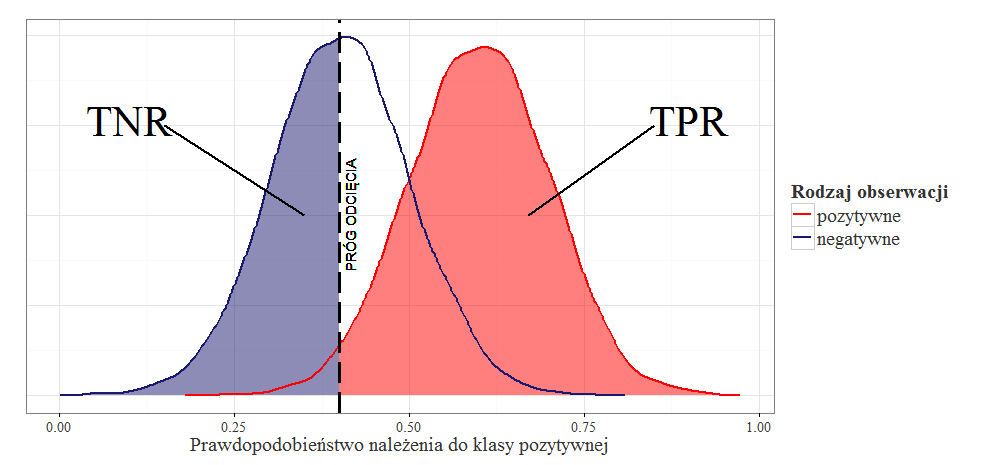
\includegraphics[width=\textwidth]{graphics/roc1.png}
    \caption{Duże TPR, ale małe TNR.}
    \label{fig:f11}
  \end{subfigure}\\
  \begin{subfigure}[h]{\textwidth}
    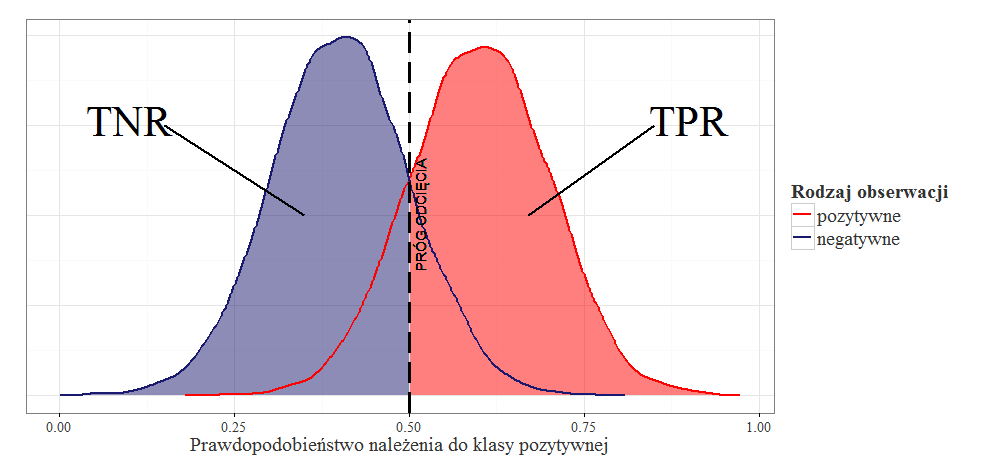
\includegraphics[width=\textwidth]{graphics/roc2.png}
    \caption{Zrównoważone TPR i TNR.}
    \label{fig:f22}
  \end{subfigure}\\
  \begin{subfigure}[h]{\textwidth}
    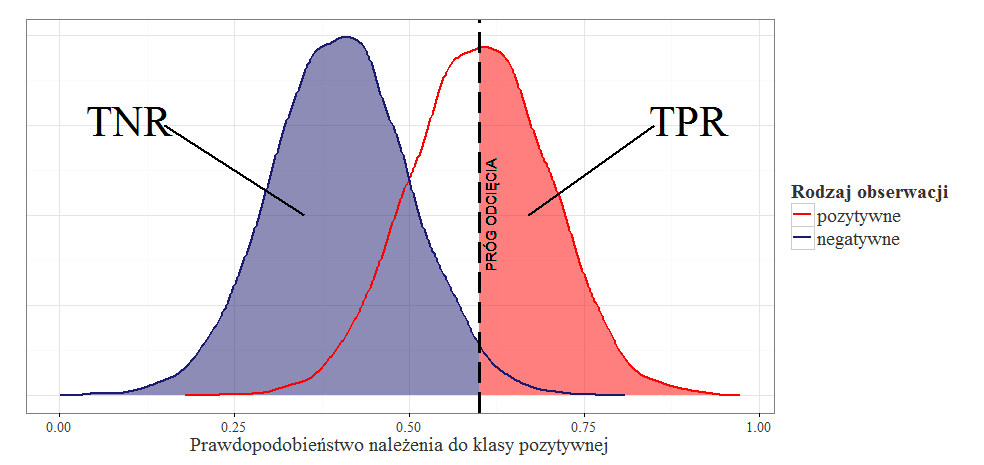
\includegraphics[width=\textwidth]{graphics/roc3.png}
    \caption{Małe TPR, ale duże TNR.}
    \label{fig:f22}
  \end{subfigure}
  \end{center}
  \caption{Sposób konstruowania krzywej ROC w przypadku dwuklasowym.}
  \label{wszystkietrzy}
\end{figure}

\vfill
\clearpage

Do stworzenia krzywej ROC, potrzebne nam będą dwa wskaźniki -- \textbf{czułość} (TPR, ang. \textit{True Positive Rate}) i \textbf{specyficzność} (TNR, ang. \textit{True Negative Rate}). Czułość definiować będziemy jako prawdopodobieństwo, że pozytywny rekord zostanie poprawnie zakwalifikowany jako pozytywny, a specyficzność jako prawdopodobieństwo, że negatywny rekord zostanie poprawnie zakwalifikowany jako negatywny. Inaczej mówiąc, czułość i specyficzność to procent poprawnie sklasyfikowanych rekordów, odpowiednio w grupie pozytywnej i negatywnej. Korzystając z tabeli jakości dopasowania (patrz Rys. \ref{tabeladopasowania}), otrzymujemy:
\begin{eqnarray*}
	TPR&=&\dfrac{TP}{TP+FN},\\
	TNR&=&\dfrac{TN}{FP+TN}.		
\end{eqnarray*}  

Ale jak stworzyć krzywą, mając tylko dwa wskaźniki? Otóż krzywa ROC to wykres punktów ($1-$TNR, TPR), wyliczonych dla różnych progów odcięcia. Czym jest zatem próg odcięcia? W większości przypadków, model generuje nam nie tylko klasę, do której powinniśmy zaklasyfikować daną obserwację, ale przede wszystkim prawdopodobieństwo, z jakim możemy coś zakwalifikować do klasy pozytywnej. Standardowo przyjmuje się, że to prawdopodobieństwo wynosi $0,5$, ale niekoniecznie musi tak być. Czasem wystarczy nam $40\%$ pewności, żeby coś zaklasyfikować jako pozytywne. Dużo tu zależy od historii, która stoi za naszymi danymi. Na przykład, gdy zajmujemy się klasyfikowaniem pacjentów na chorych i zdrowych, wolimy częściej zakwalifikować kogoś jako chorego, gdy rzeczywiście jest zdrowy, niż odwrotnie, dlatego to prawdopodobieństwo często zmniejszamy. W przypadku analizowania na przykład kampanii reklamowych, może się zdarzyć, że podniesienie progu (czyli zakwalifikowanie mniejszej liczby klientów, jako tych , do których wysłać reklamę) może znacznie zmniejszyć koszty naszej kampanii reklamowej i w rezultacie zwiększyć zysk. I właśnie ten sposób możemy zmieniać próg odcięcia. 

\begin{figure}[h]
  \begin{subfigure}[b]{0.4\textwidth}
    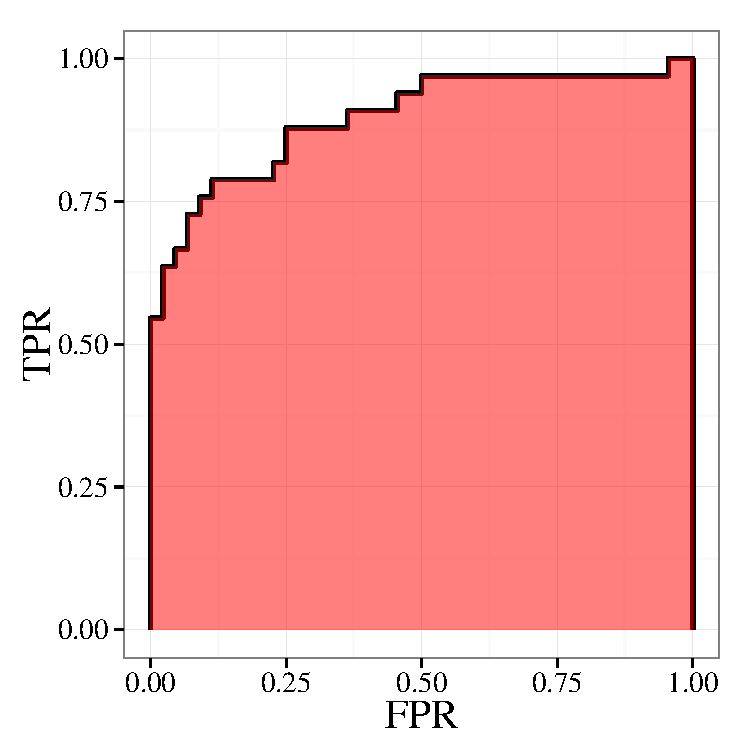
\includegraphics[width=\textwidth]{graphics/roc1.pdf}
    \caption{Standardowy sposób rysowania krzywej ROC.}
    \label{fig:f1}
  \end{subfigure}
  \hfill
  \begin{subfigure}[b]{0.4\textwidth}
    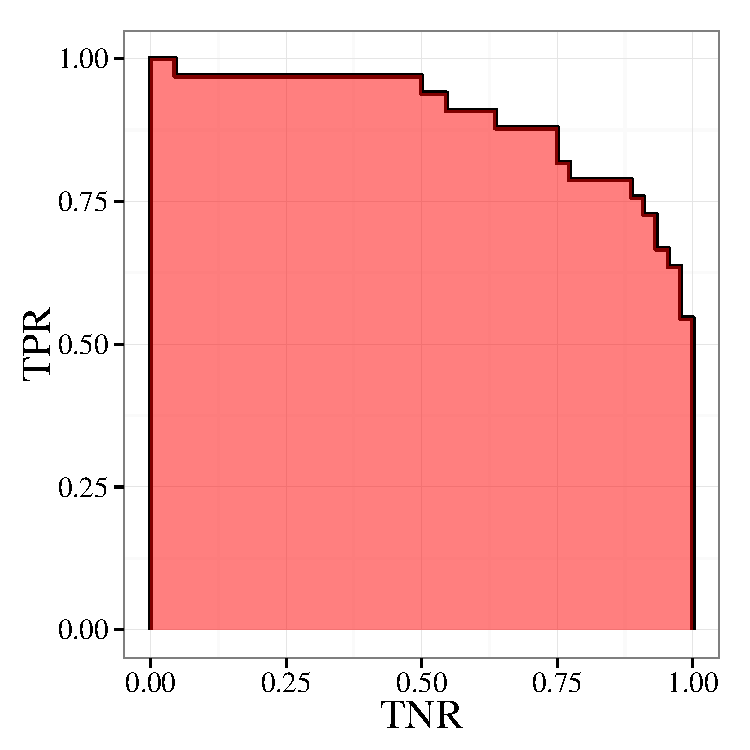
\includegraphics[width=\textwidth]{graphics/roc2.pdf}
    \caption{Krzywa ROC z TNR (zamiast FPR) na osi OX.}
    \label{fig:f2}
  \end{subfigure}
  \caption{Przykładowe krzywe ROC.}
  \label{krzyweroc}
\end{figure}

Przyjrzyjmy się rysunkowi \ref{wszystkietrzy}. Mamy tu wykresy gęstości obserwacji pozytywnych i negatywnych, w zależności od przyjętego progu odcięcia. Większość obserwacji pozytywnych osiąga około $60-$procentowe prawdopodobieństwo przynależności do klasy pozytywnej, a negatywnych $40-$procentowe prawdopodobieństwo przynależności do klasy negatywnej. Z wykresów wyraźnie widać, że poruszanie tym progiem odcięcia w prawo zwiększy nam czułość, ale zmniejszy specyficzność, natomiast poruszanie w lewo odwrotnie. Patrząc na krzywą ROC, możemy zobaczyć ich zależność od siebie na jednym wykresie i wybrać taki próg, jaki nam najbardziej odpowiada (najczęściej taki, który jest dobrym kompromisem między czułością a specyficznością). Standardowo, krzywą ROC rysuje się nie w zależności od specyficzności, tylko od jej dopełnienia (tzn. $1-$specyficzności), nazywanego FPR (ang. \textit{False Positive Rate}). My jednak, by łatwiej było nam uogólnić krzywą ROC na więcej wymiarów, zastosujemy tę mniej popularną reprezentację, czyli na osi OX będziemy przedstawiać specyficzność (patrz Rys.\ref{krzyweroc}). 

Idealna krzywa to taka, która ma duże TPR i małe FPR, tworzy zatem kwadrat jednostkowy. Zła krzywa, czyli taka, która powstaje, gdy model daje losowe wyniki, to taka, która jest przekątną tego kwadratu. Ponieważ, patrząc na dwie często wielokrotnie przecinające się krzywe ROC, odpowiadające różnym modelom, ciężko jest stwierdzić, która krzywa jest lepsza, wprowadzono współczynnik AUC, czyli pole pod tą krzywą, który pozwala łatwiej to ocenić. Idealny model ma współczynnik AUC równy $1$, a model losowy charakteryzuje się AUC równym $0,5$. Na rysunku \ref{krzyweroc} łatwo widać, że w naszym przypadku (czyli z inaczej zdefiniowaną osią OX) współczynnik AUC definiuje się identycznie.       

\section{Krzywa ROC w przypadku regresji porządkowej}

\begin{figure}[h]
	\begin{center}
  \begin{subfigure}[h]{\textwidth}
    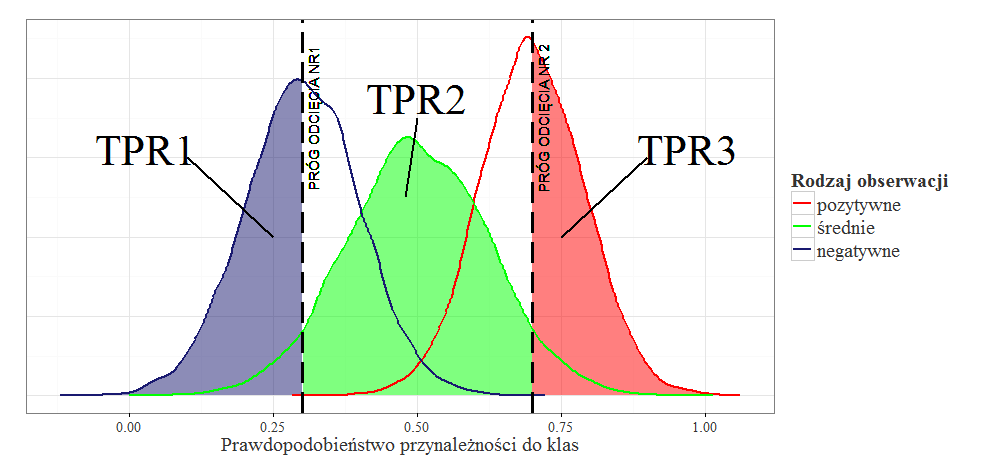
\includegraphics[width=\textwidth]{graphics/roc_trzy1.png}
  \end{subfigure}\\
  \begin{subfigure}[h]{\textwidth}
    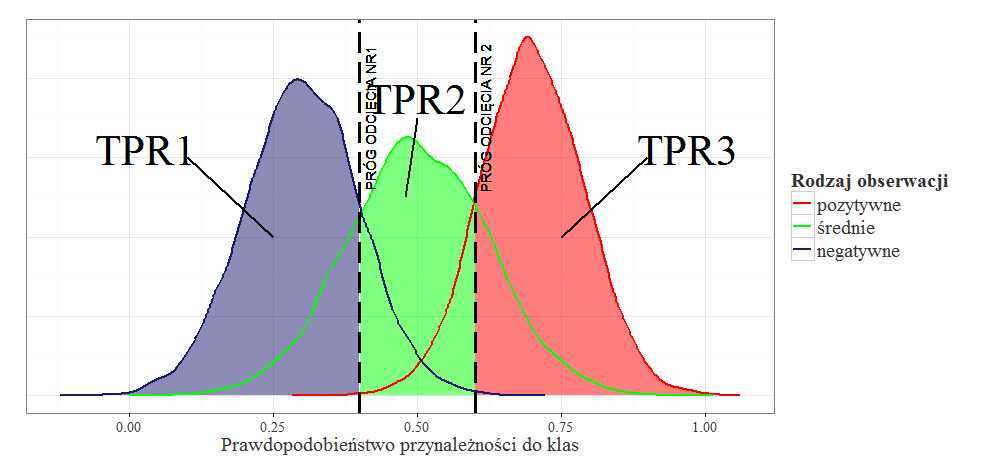
\includegraphics[width=\textwidth]{graphics/roc_trzy2.png}
  \end{subfigure}
  \end{center}
  \caption{Sposób konstruowania krzywej ROC w przypadku trzyklasowym.}
  \label{trzyklasowy}
\end{figure}

W przypadku regresji porządkowej dochodzi problem wielowymiarowości. Przede wszystkim nie mamy tu podziału na klasę pozytywną i negatywną, jak więc stworzyć współczynnik FPR? Można próbować robić to parami tzn. traktować jedną z klas jako pozytywną, a pozostałe połączyć w jedną i traktować jako negatywną. Robiąc w ten sposób z każdą klasą, otrzymamy $r$ (bo tyle jest możliwych poziomów zmiennej odpowiedzi) krzywych ROC, a tym samym $r$ współczynników AUC. Jako ostateczne AUC przyjmuje się wtedy średnią z nich. Nie jest to jednak dobry wskaźnik. Może się bowiem zdarzyć tak, że współczynnik między środkowymi klasami wyjdzie duży, natomiast ten między klasami skrajnymi słaby, tworząc tym samym nienajgorszą średnią. Nie jest to dobre, gdyż często zależy nam na dobrym odróżnieniu właśnie klas skrajnych. Wyobraźmy sobie, że chcemy sprawdzić, czy komuś spodobałaby się sprzedawana przez nas książka. Możliwe odpowiedzi to: bardzo mi się podoba, podoba mi się, nie mam zdania, nie podoba mi się, bardzo mi się nie podoba. Jasne jest, że wolelibyśmy oddzielić klientów, którym bardzo spodobałaby się książka od tych, którym bardzo by się nie spodobała, a nie na przykład tych, którym by się nie spodobała od tych, którym by się bardzo nie spodobała. Żeby udało nam się poradzić sobie z takim problemem, trzeba spojrzeć na niego globalnie.   

Opisując krzywą ROC w przypadku dwuklasowym powiedzieliśmy sobie, że będziemy rozważać nie zależność TPR od FPR, ale TPR od TNR. Dlaczego? Właśnie po to, żebyśmy teraz mogli ją łatwiej uogólnić. Zarówno TPR, jak i TNR jest to procent poprawnie sklasyfikowanych odpowiednio pozytywnych bądź negatywnych obserwacji. Nic nie staje zatem na przeszkodzie, by stworzyć $r$ takich współczynników ($\text{TPR}1, \ldots, \text{TPR}r$), każdy odpowiadający procentowi poprawnie sklasyfikowanych obserwacji z $i-$tej klasy. Przyjmując różne progi odcięcia (patrz Rys. \ref{trzyklasowy}), których tym razem będzie $r-1$, możemy narysować krzywą ROC, a raczej pewną hiperpowierzchnię. Oczywiście jest to możliwe tylko w przypadku trzyklasowym (patrz Rys. \ref{3d}), ale rysunek taki i tak jest raczej mało czytelny. 

\begin{figure}[h]
\begin{center}
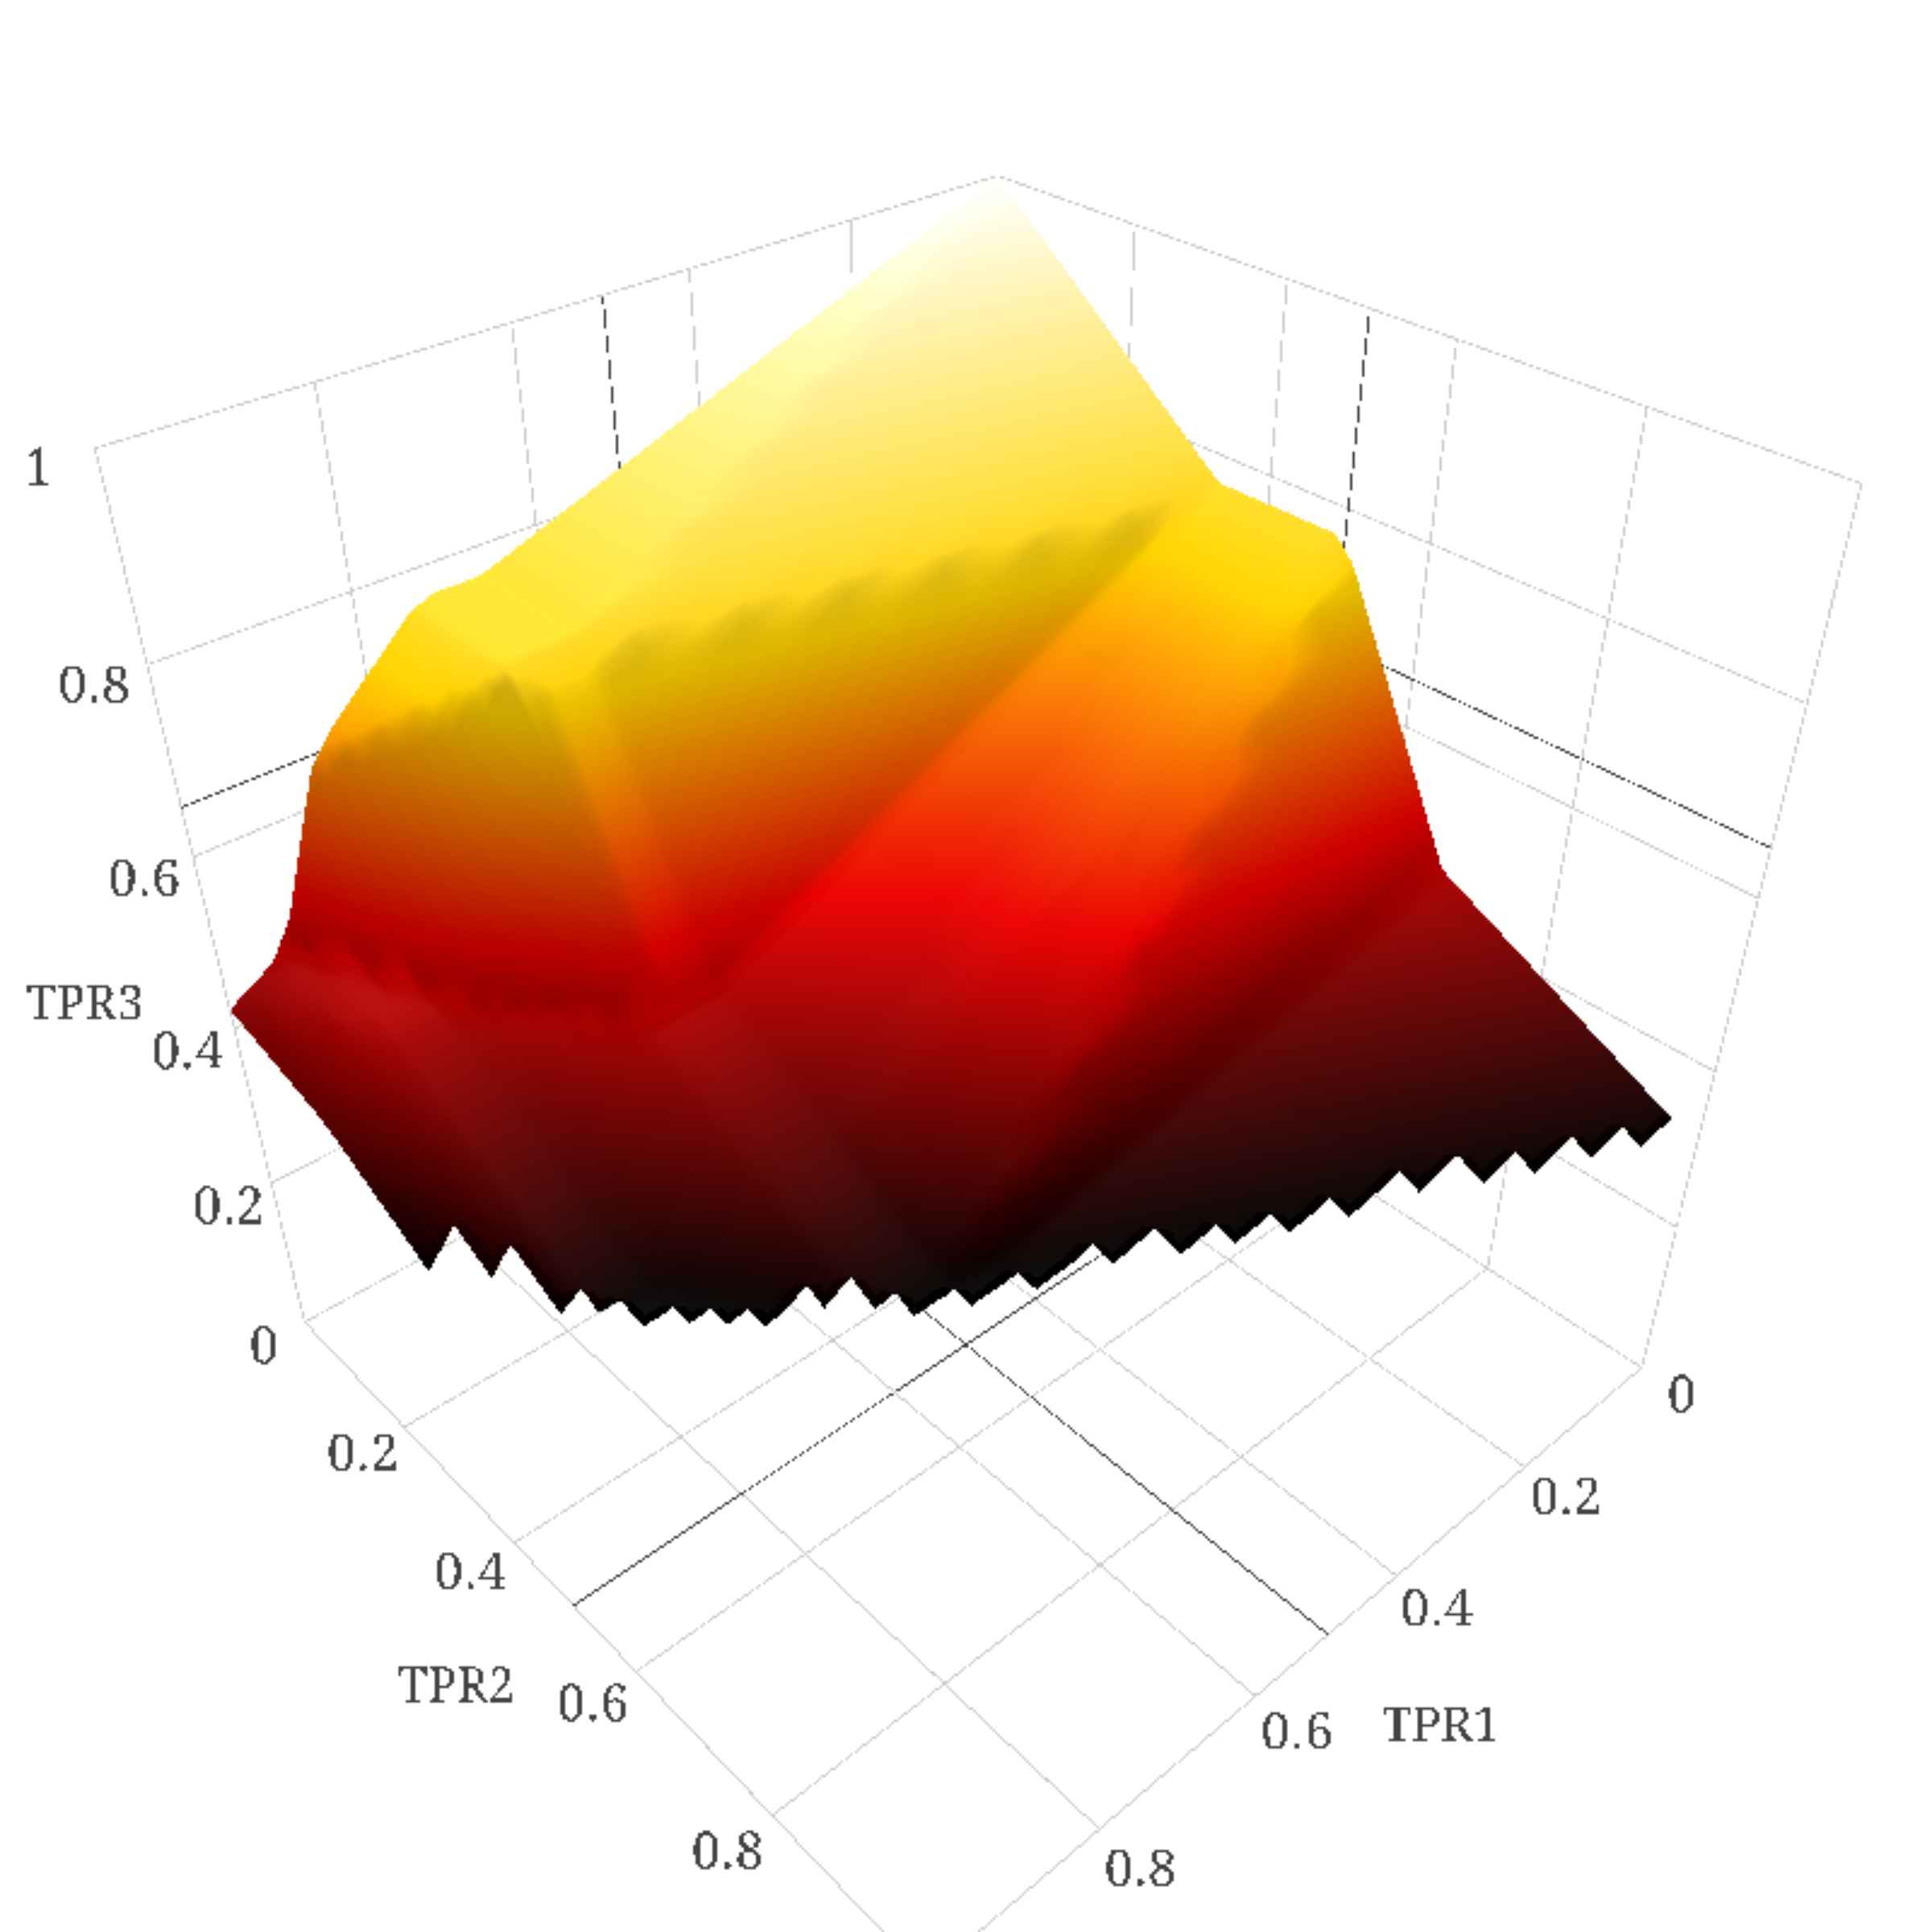
\includegraphics[scale=0.5]{graphics/roc3d.png}
\end{center}
\caption{Krzywa ROC w przypadku trzyklasowym.}
\label{3d}
\end{figure}

\section{Współczynnik VUS}

Po co zatem tworzyć wielowymiarową krzywą ROC, skoro i tak trudno cokolwiek z niej odczytać? Otóż głównie po to, by otrzymać współczynnik AUC, który, będąc konkretną liczbą, jest znacznie prostszy w interpretacji. W przypadku więcej niż dwuwymiarowym będziemy go nazywać VUS (ang. \textit{Volume Under the Surface}). 

Jako, że liczenie objętości pod hiperpłaszczyzną jest numerycznie raczej trudnym zadaniem, w celu wyliczenia współczynnika VUS, skorzystamy z jego nieco innej interpretacji niż tylko pole pod krzywą ROC. Wróćmy znów do przypadku dwuklasowego i przyjrzyjmy się wykresowi \ref{fig:f2}. Na osi OY mamy współczynnik TNR, czyli prawdopodobieństwo, że wyestymujemy klasę negatywną pod warunkiem, że klasa rzeczywiście jest negatywna. Równoważnie, można to zapisać jako prawdopodobieństwo, że prawdopodobieństwo odpowiadające negatywnej obserwacji jest mniejsze niż pewien próg odcięcia. Analogicznie TPR to prawdopodobieństwo, że prawdopodobieństwo odpowiadające pozytywnej obserwacji jest większe niż próg odcięcia. Łącząc oba wyniki otrzymamy, że współczynnik AUC to nic innego tylko prawdopodobieństwo, że losowo wybrana pozytywna obserwacja będzie mieć wyższe prawdopodobieństwo niż losowo wybrana negatywna obserwacja. Innymi słowy, będą one dobrze uporządkowane. Łatwo to już uogólnić na więcej wymiarów. Interesować nas będzie pewna estymacja tego prawdopodobieństwa. Łatwo można zauważyć, że będzie nią tzw. statystyka $U$  Manna–Whitney'a–Wilcoxona (por. \cite{roc1}, \cite{roc2}), czyli wyrażenie:

\begin{equation}\label{dop3}
VUS = \dfrac{1}{n_1n_2\cdot\ldots\cdot n_r}\sum_{i_1=1}^{n_1}\sum_{i_2=1}^{n_2}\ldots\sum_{i_r=1}^{n_r}\mathbb{I}_{\lbrace f(\mathbf{x}_{i_1}^1)<\ldots<f(\mathbf{x}_{i_r}^r)\rbrace},
\end{equation}
gdzie $\textbf{x}_i^j$ oznacza $i-$ty wektor cech $\mathbf{x}$ o prawdziwej klasie $j$, $n_i$ to liczba obserwacji zaklasyfikowanych przez nas jako klasa $i$, a $f$ to pewna funkcja, która zwraca liczbę rzeczywistą, mającą estymować uporządkowanie obserwacji (w większości przypadków, będzie to prawdopodobieństwo zwracane na koniec).

Krzywa ROC i współczynnik VUS jest więc dość prostym, bardzo łatwo interpretowalnym i pomocnym narzędziem do oceny jakości modelu i podejmowania decyzji, który model jest najlepszy. Największą jego wadą wydaje się konieczność znania prawdopodobieństw przynależności do klas (lub po prostu funkcji, która pozwoli nasze obserwacje uporządkować), a nie każda metoda takie prawdopodobieństwa zwraca (np. nie robią tego sieci neuronowe). Trzeba wtedy odwołać się do prostszych metod (takich jak procent poprawności dopasowania lub czułość). Większość modeli oferuje jednak taką możliwość, więc niewątpliwie warto z tego narzędzia diagnostycznego korzystać.

\chapter{Porównanie metod modelowania i współczynników diagnostycznych}

W poprzednich rozdziałach poznaliśmy różne techniki radzenia sobie z problemem regresji porządkowej. Znamy już również techniki oceny klasyfikatorów. Spróbujmy teraz zobaczyć, jak na rzeczywistych danych zachowuje się każda z poznanych metod. 

\section{Opis danych}

\begin{figure}[h!t]
\begin{center}
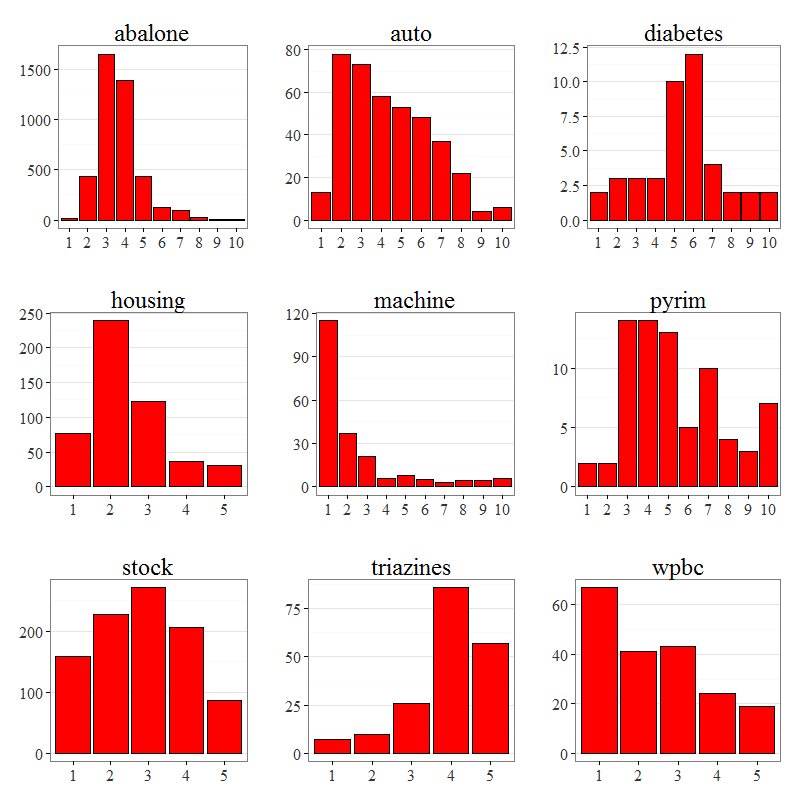
\includegraphics[scale=0.6]{graphics/rozklad_odpowiedzi.png}
\end{center}
\caption{Rozkłady odpowiedzi poszczególnych zbiorów danych.}
\label{rozkladdanych}
\end{figure}

Do dyspozycji mamy dziewięć zbiorów (\textit{abalone, auto, diabetes, housing, machine, pyrim, stock, triazines} oraz \textit{wpbc}) o różnej liczbie klas ($5$ lub $10$), różnej liczbie obserwacji oraz różnym rozkładzie klas (patrz Rys. \ref{rozkladdanych}). Zbiory znaleźć można tu: \cite{zbiorki}. 

Każdy ze zbiorów został losowo podzielony na zbiór treningowy (do budowy modelu) i zbiór testowy (do oceny jakości modelu) w proporcji $7:3$. Następnie, na każdym zbiorze treningowym zbudowany został każdy z pięciu modeli (model proporcjonalnych szans, model oparty o procesy gaussowskie, model Franka i Halla, sieci neuronowe oraz SVM) i przetestowany na zbiorze testowym. Dla każdego zbioru i każdej metody otrzymaliśmy współczynniki VUS, PPK i ABSerr (por. równania \ref{dop1}, \ref{dop2}, \ref{dop3}). Wszystkie wyniki zobaczyć można w tabeli \ref{wyniki}.

\begin{comment}
\begin{table}[h!t]
\centering
\begin{tabular}{rrrrrrr}
  &   & \rotatebox{70}{Procesy gaussowskie} & \rotatebox{70}{\parbox{35mm}{Model proporcjonalnych szans}} & \rotatebox{70}{Sieci neuronowe} &\rotatebox{70}{Metoda Franka i Halla} & \rotatebox{70}{\parbox{40mm}{Wektory maszyn\\ podpierających (SVM)}} \\ 
  \hline
\multirow{3}{15mm}{abalone} & VUS [\%] & 0,00 & 0,00 & -- & 0,00 & 0,00 \\ 
   & PPK [\%] & 56,38 & 55,18 & \color{red}{56,86} & 55,18 & 56,30 \\ 
   & ABSerr & 0,55 & 0,55 & \color{red}{0,51} & 0,55 & 0,52 \\ 
   \hline
\multirow{3}{15mm}{auto} & VUS [\%] & \color{red}{3,54} & 1,13 & -- & 0,25 & 0,81 \\ 
   & PPK [\%] & 37,29 & \color{red}{49,15} & 48,31 & 43,22 & 38,98 \\ 
   & ABSerr & 1,08 & \color{red}{0,63} & 0,66 & 0,73 & 0,90 \\ 
   \hline
\multirow{3}{15mm}{diabetes} & VUS [\%] & 5,00 & 5,00 & -- & \color{red}{15,00} & 5,00 \\ 
   & PPK [\%] & \color{red}{23,08} & \color{red}{23,08} & \color{red}{23,08} & 15,38 & \color{red}{23,08} \\ 
   & ABSerr & 1,46 & 1,31 & \color{red}{1,23} & \color{red}{1,23} & 1,38 \\ 
   \hline
\multirow{3}{15mm}{housing} & VUS [\%] & 54,46 & \color{red}{55,31} & -- & 42,06 & 51,33 \\ 
   & PPK [\%] & 67,11 & 67,11 & \color{red}{75,00} & 72,37 & 72,37 \\ 
   & ABSerr & 0,36 & 0,35 & \color{red}{0,26} & 0,28 & 0,29 \\ 
   \hline
\multirow{3}{15mm}{machine} & VUS [\%] & 0,00 & 0,00 & -- & 0,00 & 0,00 \\ 
   & PPK [\%] & 57,14 & \color{red}{68,25} & 66,67 & 66,67 & 60,32 \\ 
   & ABSerr & 1,17 & 0,52 & \color{red}{0,51} & 0,67 & 0,73 \\ 
   \hline
\multirow{3}{15mm}{pyrim} & VUS [\%] & \color{red}{1,11} & 0,00 & -- & 0,56 & 0,93 \\ 
   & PPK [\%] & 21,74 & 8,70 & \color{red}{52,17} & 30,43 & 47,83 \\ 
   & ABSerr & 1,30 & 1,65 & \color{red}{0,91} & \color{red}{0,91} & 0,96 \\ 
   \hline
\multirow{3}{15mm}{stock} & VUS [\%] & 53,97 & 73,12 & -- & 56,53 & \color{red}{96,01} \\ 
   & PPK [\%] & 58,95 & 72,63 & 83,16 & 81,40 & \color{red}{91,58} \\ 
   & ABSerr & 0,42 & 0,28 & 0,18 & 0,19 & \color{red}{0,08} \\ 
   \hline
\multirow{3}{15mm}{triazines} & VUS [\%] & 1,84 & 1,83 & -- & \color{red}{5,45} & 1,96 \\ 
   & PPK [\%] & 51,79 & 39,29 & 39,29 & \color{red}{53,57} & 51,79 \\ 
   & ABSerr & 0,64 & 0,91 & 0,71 & \color{red}{0,61} & 0,64 \\ 
   \hline
\multirow{3}{15mm}{wpbc} & VUS [\%] & \color{red}{4,44} & 3,99 & -- & 0,63 & 1,88 \\ 
   & PPK [\%] & 33,90 & 30,51 & \color{red}{35,59} & 28,81 & 28,81 \\ 
   & ABSerr & 1,12 & 1,25 & \color{red}{0,86} & 1,02 & 0,92 \\ 
   \hline
\end{tabular}
\caption{Tabela wyników. Na czerwono zaznaczony jest najlepszy wynik dla każdego wskaźnika każdego zbioru. Dla sieci neuronowych nie da się niestety obliczyć współczynnika VUS.}
\label{wyniki} 
\end{table}
\end{comment}



\section{Analiza wyników}

\subsection*{Słaby współczynnik VUS}

Pierwszą rzeczą, która rzuca się w oczy, patrząc na tabelę wyników (Tabela \ref{wyniki}), jest niska jakość współczynnika VUS. W większości przypadków jest on zerowy lub bardzo mały. Przypomnijmy, że reprezentuje on pewne prawdopodobieństwo, wobec czego już nawet wynik $50\%$ byłby nienajlepszy, a co dopiero $0\%$. Sensowny wynik współczynnika VUS zobaczyć możemy tak naprawdę jedynie w przypadku zbiorów \textit{housing} i \textit{stock}. Warto więc zadać sobie pytanie, dlaczego tak się dzieje? Żeby zrozumieć to "dziwne" zachowanie współczynnika VUS, przeanalizujmy dwa poniższe przykłady.

Załóżmy, że chcemy przyporządkować klasy pewnym obserwacjom ze zbioru testowego. Nich zbiorem klas będzie $\lbrace 1, \ldots, 5\rbrace$. Dopasowaliśmy pewien model, który działa w ten sposób, że dla danej nowej obserwacji wylicza najpierw wartość pewnej funkcji rzeczywistej $f$, a następnie, korzystając z pewnych progów, dzieli zbiór liczb rzeczywistych na pięć klas. W zależności od tego, między jakimi dwoma progami znajdzie się wartość funkcji $f$ dla danej obserwacji, to taką estymowaną klasę $\hat{y}$ jej przydzielimy. Funkcja $f$ oraz wartości progów zostały nauczone podczas budowy modelu. 

Rozważmy najpierw przypadek z rysunku \ref{vus01}. Wszystkie klasy -- oprócz jednej -- zostały prawidłowo przyporządkowane. Podkreślmy, że pomyliliśmy się tylko w jednym przypadku. Co prawda pomyłka jest poważna (bo przyporządkowaliśmy skrajnie różną wartość), ale wciąż jest to tylko jeden przypadek. Korzystając ze wzoru \ref{dop3} i pamiętając, że VUS to procent dobrze uporządkowanych , w naszym przypadku, piątek $(1, 2, 3, 4, 5)$, bardzo łatwo zauważyć, że współczynnik VUS w naszym przypadku wyniesie $0$. Wynika to z faktu, że jedyna piątka wśród zmiennej odpowiedzi uplasowała się na samum początku.

Ktoś mógłby powiedzieć, że pomylenie skrajnych wartości jest poważnym błędem, więc dobrze, że VUS wyszedł taki słaby. Przyjrzyjmy się zatem przykładowi z rysunku \ref{vus02}. Tutaj sytuacja jest podobna - tym razem również została pomylona tylko jedna wartość (obserwacja o rzeczywistym nr 5 dostała nr 4). Tym razem błąd jest niewielki, a nie skrajny, jak w poprzednim przykładzie, i -- chciałoby się powiedzieć -- dopuszczalny i nieszkodliwy. Jednak w tym przypadku również nie znajdziemy ani jednej dobrze posortowanej piątki, współczynnik VUS wyniesie więc $0$.      

\begin{figure}[h]
\begin{subfigure}{0.5\textwidth}
\begin{center}
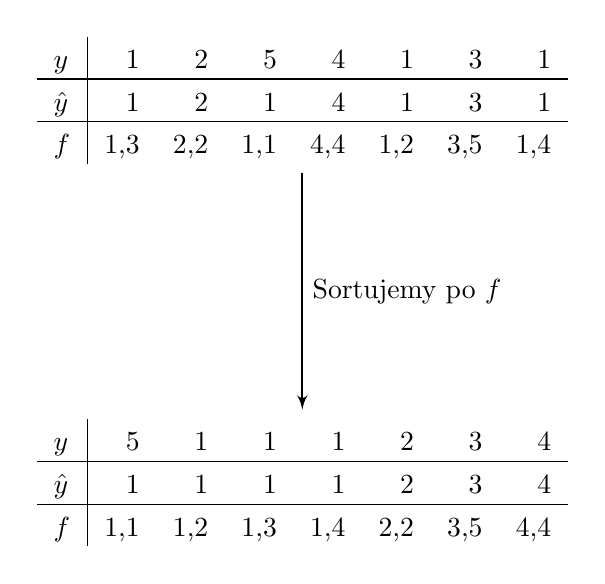
\begin{tikzpicture}
\node(gora){
\begin{tabular}{l|rrrrrrr}
 $y$ & 1 & 2 & 5 & 4 & 1 & 3 & 1\\
\hline
 $\hat{y}$ & 1 & 2 & 1 & 4 & 1 & 3 & 1\\
\hline
 $f$ & 1,3 & 2,2 & 1,1 & 4,4 & 1,2 & 3,5 & 1,4\\
\end{tabular}
};
\node[below=3cm of gora](dol){
\begin{tabular}{l|rrrrrrr}
 $y$ & 5 & 1 & 1 & 1 & 2 & 3 & 4\\
\hline
 $\hat{y}$ & 1 & 1 & 1 & 1 & 2 & 3 & 4\\
\hline
 $f$ & 1,1 & 1,2 & 1,3 & 1,4 & 2,2 & 3,5 & 4,4\\
\end{tabular}
};
\path[draw, -latex',thick](gora) -- node[midway, right] {Sortujemy po $f$} (dol);		
\end{tikzpicture}
\end{center}
\caption{Przypadek, w którym źle sklasyfikowana jest tylko jedna obserwacja. Zamiast klasy nr $5$, została przyporządkowana klasa nr $1$.}
\label{vus01}
\end{subfigure}
\hspace{1cm}
\begin{subfigure}{0.5\textwidth}
\begin{center}
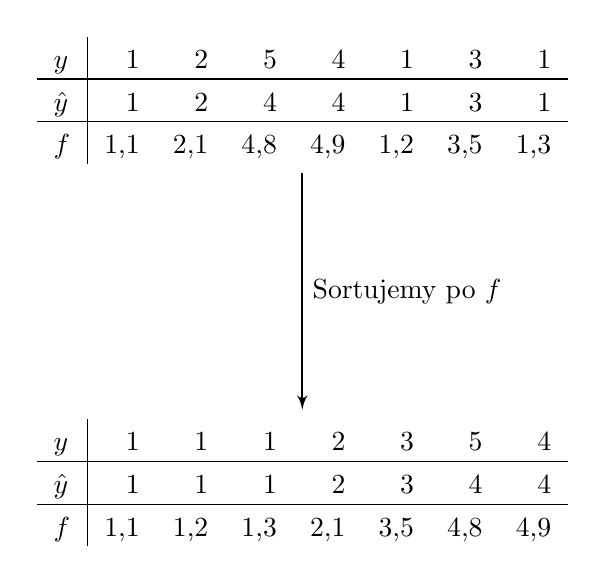
\begin{tikzpicture}
\node(gora){
\begin{tabular}{l|rrrrrrr}
 $y$ & 1 & 2 & 5 & 4 & 1 & 3 & 1\\
\hline
 $\hat{y}$ & 1 & 2 & 4 & 4 & 1 & 3 & 1\\
\hline
 $f$ & 1,1 & 2,1 & 4,8 & 4,9 & 1,2 & 3,5 & 1,3\\
\end{tabular}
};
\node[below=3cm of gora](dol){
\begin{tabular}{l|rrrrrrr}
 $y$ & 1 & 1 & 1 & 2 & 3 & 5 & 4\\
\hline
 $\hat{y}$ & 1 & 1 & 1 & 2 & 3 & 4 & 4\\
\hline
 $f$ & 1,1 & 1,2 & 1,3 & 2,1 & 3,5 & 4,8 & 4,9\\
\end{tabular}
};
\path[draw, -latex',thick](gora) -- node[midway, right] {Sortujemy po $f$} (dol);	
\end{tikzpicture}
\end{center}
\caption{Przypadek, w którym źle sklasyfikowana jest tylko jedna obserwacja. Zamiast klasy nr $5$, została przyporządkowana klasa nr $4$.}
\label{vus02}
\end{subfigure}
\caption{Tabele pokazują przykładowe zbiory testowe. W kolumnach przedstawione są kolejne obserwacje. $y$ reprezentuje prawdziwą klasę, a $\hat{y}$ oszacowaną przez nas klasę na podstawie wartości funkcji rzeczywistej $f$. Następnie kolumny tabeli są sortowane według wartości tej funkcji.}
\end{figure}

Współczynnik VUS, który ma bardzo ładną interpretację i znakomicie sprawdza się w przypadku klasyfikacji dwuetykietowej, w przypadku regresji porządkowej nie spełnia niestety swojej roli. Przypomnijmy sobie jeszcze raz, jaka ta rola powinna być. W przeciwieństwie do PPK, VUS nie pokazuje, ile obserwacji zostało poprawnie sklasyfikowanych. Wręcz możliwa jest sytuacja, że VUS wyniesie $100\%$, mimo że wszystkie obserwacje zaklasyfikowaliśmy źle. Co więc daje nam ten wskaźnik? Daje nam pojęcie, czy obserwacje zostały poprawnie posortowane. Patrząc na powyższe dwa przykłady wyraźnie widać, że -- szczególnie w przypadku nierównolicznych klas -- ta intuicja nie do końca zgadza się z rzeczywistością.

\subsection*{Współczynnik SB (Sortowanie Bąbelkowe)}

Chciałabym więc zaproponować współczynnik, który posiadałby interpretację współczynnika VUS i jednocześnie rozwiązywał problem jego słabej jakości. Nazwałam go SB (od sortowania bąbelkowego). 

Idea jest bardzo prosta (patrz Algorytm \ref{algo:bubble_sort}) -- podobnie jak w przypadku VUS, sortujemy rzeczywiste klasy obserwacji ze zbioru testowego malejąco. Następnie, stosując algorytm sortowania bąbelkowego, zliczamy ile przestawień sąsiednich wyrazów będzie potrzeba, by poprawnie uporządkować wejściowy wektor obserwacji. Porównujemy to do maksymalnej liczby przestawień (czyli do takiej, która jest potrzebna do rosnącego posortowania tego samego wektora, lecz uporządkowanego malejąco). W rezultacie otrzymujemy liczbę wahającą się od $0$, reprezentującego najgorszy przypadek, do $1$, reprezentującej przypadek najlepszy. 

\begin{algorithm}
\begin{algorithmic}
\STATE
\STATE \textbf{function} \texttt{liczba\_przestawien}$(wektor)$
\bindent
\STATE $ile\_zamian := 0$ 
\FOR {$j$ in $length(wektor):2$}
    \FOR {$i$ in $1:(j-1)$ }
        \IF {$wektor[i]>wektor[i+1]$}
            \STATE zamień $wektor[i]$ i $wektor[i+1]$
            \STATE $ile\_zamian := ile\_zamian+1$
        \ENDIF
    \ENDFOR
\ENDFOR
\eindent
\STATE \textbf{end function}
\STATE
\STATE $w1$ jest wektorem klas posortowanym ze względu na wartość funkcji $f$
\STATE $w2$ jest wektorem klas posortowanym malejąco
\STATE
\STATE \textbf{return} $1-(\texttt{liczba\_przestawien}(w1)/\texttt{liczba\_przestawien}(w2))$

\end{algorithmic}
\caption{Wyznaczanie współczynnika SB}
\label{algo:bubble_sort}
\end{algorithm}

Widać więc, że -- podobnie jak VUS -- SB nie bierze pod uwagę dokładnej wartości przypisanej klasy, jedynie ich kolejność. Nie ma jednak tej wady, że jedna lekko źle zaklasyfikowana obserwacja może sprawić, że zostanie on wyzerowany. Niestety -- podobnie jak VUS -- nie da się go zastosować do metod, których krokiem pośrednim nie jest wyznaczenie pomocniczej funkcji $f$, co jest jego niewątpliwą wadą.

Wróćmy znów do przykładów z rysunku \ref{vus01} i \ref{vus02}. W pierwszym z nich współczynnik SB wynosi $67\%$, w drugim zaś $94\%$, co niejako zgadza się z naszą intuicją. Podobnie, w przypadku tabeli \ref{wyniki}, gdzie współczynnik SB, w przeciwieństwie do VUS, daje nam już jakąś informację.

Warto wreszcie podkreślić, że nie trzeba stosować tylko jednego współczynnika. Czasem warto spojrzeć zarówno na PPK, VUS i SB i zastanowić się, na czym najbardziej nam zależy -- na precyzji czy na kolejności dopasowania. Może czasem warto zrezygnować z doskonałej kolejności, by zyskać dużo większą precyzję? I odwrotnie. To już kwestia indywidualnego przypadku i charakteru danych. 

\begin{table}[th!]
\centering
\begin{tabular}{rrrrrrr}
  &   & \rotatebox{90}{\parbox{25mm}{\hspace{2cm}\\ \hspace{2cm}\\Procesy\\ gaussowskie}} & \rotatebox{90}{\parbox{25mm}{\hspace{2cm}\\ \hspace{2cm}\\Model\\ proporcjonalnych \\szans}} & \rotatebox{90}{\parbox{25mm}{\hspace{2cm}\\ \hspace{2cm}\\Sieci\\ neuronowe}} &\rotatebox{90}{\parbox{25mm}{\hspace{2cm}\\ \hspace{2cm}\\Metoda\\ Franka \\i Halla}} & \rotatebox{90}{\parbox{25mm}{\hspace{2cm}\\ \hspace{2cm}\\Wektory\\ maszyn\\ podpierających\\ (SVM)}} \\ 
  \hline
\multirow{4}{15mm}{abalone} & VUS [\%] & 0,00 & 0,00 & -- & 0,00 & 0,00 \\ 
   & PPK [\%] & 56,38 & 55,18 & \color{red}{56,86} & 55,18 & 56,30 \\ 
   & ABS & 0,55 & 0,55 & \color{red}{0,51} & 0,55 & 0,52 \\ 
   & SB [\%] & 83,45 & 83,66 & -- & 76,45 & \color{red}{85,34} \\ 
   \hline
\multirow{4}{15mm}{auto} & VUS [\%] & \color{red}{3,54} & 1,13 & -- & 0,25 & 0,81 \\ 
   & PPK [\%] & 37,29 & \color{red}{49,15} & 48,31 & 43,22 & 38,98 \\ 
   & ABS & 1,08 & \color{red}{0,63} & 0,66 & 0,73 & 0,90 \\ 
   & SB [\%] & \color{red}{94,16} & 94,12 & -- & 88,77 & 87,96 \\ 
   \hline
\multirow{4}{15mm}{diabetes} & VUS [\%] & 5,00 & 5,00 & -- & \color{red}{15,00} & 5,00 \\ 
   & PPK [\%] & \color{red}{23,08} & \color{red}{23,08} & \color{red}{23,08} & 15,38 & \color{red}{23,08} \\ 
   & ABS & 1,46 & 1,31 & \color{red}{1,23} & \color{red}{1,23} & 1,38 \\ 
   & SB [\%] & 51,61 & 51,61 & -- & \color{red}{72,58} & 40,32 \\ 
   \hline
\multirow{4}{15mm}{housing} & VUS [\%] & 54,46 & \color{red}{55,31} & -- & 42,06 & 51,33 \\ 
   & PPK [\%] & 67,11 & 67,11 & \color{red}{75,00} & 72,37 & 72,37 \\ 
   & ABS & 0,36 & 0,35 & \color{red}{0,26} & 0,28 & 0,29 \\ 
   & SB [\%] & 91,86 & \color{red}{92,25} & -- & 86,92 & 91,98 \\ 
   \hline
\multirow{4}{15mm}{machine} & VUS [\%] & 0,00 & 0,00 & -- & 0,00 & 0,00 \\ 
   & PPK [\%] & 57,14 & \color{red}{68,25} & 66,67 & 66,67 & 60,32 \\ 
   & ABS & 1,17 & 0,52 & \color{red}{0,51} & 0,67 & 0,73 \\ 
   & SB [\%] & 90,50 & \color{red}{92,87} & -- & 91,34 & 87,36 \\ 
   \hline
\multirow{4}{15mm}{pyrim} & VUS [\%] & \color{red}{1,11} & 0,00 & -- & 0,56 & 0,93 \\ 
   & PPK [\%] & 21,74 & 8,70 & \color{red}{52,17} & 30,43 & 47,83 \\ 
   & ABS & 1,30 & 1,65 & \color{red}{0,91} & \color{red}{0,91} & 0,96 \\ 
   & SB [\%] & 81,82 & 74,09 & -- & 80,00 & \color{red}{82,73} \\ 
   \hline
\multirow{4}{15mm}{stock} & VUS [\%] & 53,97 & 73,12 & -- & 56,53 & \color{red}{96,01} \\ 
   & PPK [\%] & 58,95 & 72,63 & 83,16 & 81,40 & \color{red}{91,58} \\ 
   & ABS & 0,42 & 0,28 & 0,18 & 0,19 & \color{red}{0,08} \\ 
   & SB [\%] & 93,07 & 95,51 & -- & 94,31 & \color{red}{99,42} \\ 
   \hline
\multirow{4}{15mm}{triazines} & VUS [\%] & 1,84 & 1,83 & -- & \color{red}{5,45} & 1,96 \\ 
   & PPK [\%] & 51,79 & 39,29 & 39,29 & \color{red}{53,57} & 51,79 \\ 
   & ABS & 0,64 & 0,91 & 0,71 & \color{red}{0,61} & 0,64 \\ 
   & SB [\%] & 62,86 & 45,58 & -- & \color{red}{66,46} & 58,33 \\ 
   \hline
\multirow{4}{15mm}{wpbc} & VUS [\%] & \color{red}{4,44} & 3,99 & -- & 0,63 & 1,88 \\ 
   & PPK [\%] & 33,90 & 30,51 & \color{red}{35,59} & 28,81 & 28,81 \\ 
   & ABS & 1,12 & 1,25 & \color{red}{0,86} & 1,02 & 0,92 \\ 
   & SB [\%] & \color{red}{67,59} & 61,29 & -- & 62,67 & 57,53 \\ 
   \hline
\end{tabular}
\caption{Tabela wyników. Na czerwono zaznaczony jest najlepszy wynik dla każdego wskaźnika każdego zbioru. Dla sieci neuronowych nie da się niestety obliczyć współczynnika VUS ani SB.}
\label{wyniki} 
\end{table}

\subsection*{Dalsze wnioski}

Wróćmy do wniosków płynących z symulacji.

Warto zwrócić uwagę na niespodziewanie dobre zachowanie sieci neuronowych. Osiągają one najlepszy procent poprawnej klasyfikacji w $56\%$ zbiorów, a w $22\%$ niewiele odbiegają  od najlepszego wyniku. Niestety nie możemy tutaj porównać współczynnika VUS ani SB. 

No i w końcu, widać wyraźnie, że nie ma jednej najlepszej metody. Każda analizowana metoda ,,wygrywa" na którymś ze zbiorów, każda ma swoje wady i zalety.

\begin{comment}

Analizując powyższe wyniki, nasuwają się na myśl ciekawe pytania. Przede wszystkim dlaczego współczynnik VUS wychodzi taki słaby? Czy może zależy to od liczby klas zmiennej odpowiedzi? Czy każda z metod też od tego zależy? W następnym podrozdziale spróbujemy sobie na te pytania odpowiedzieć. 



%\section{Dane o różnej liczbie klas}

Weźmy pod uwagę zbiór danych \textit{machine}. Zmienna odpowiedzi jest tu zmienną ciągłą, która w powyższej analizie została -- w sposób lekko szutuczny -- zdyskretyzowana. Zróbmy teraz to samo, ale dyskretyzując zbiór na, odpowiednio, $3$, $5$, $7$, i $10$ klas. By sprawdzić dodatkowo, czy różnice zależą od liczby klas, czy może jednak od ich liczności, rozważać będziemy dwa rodzaje dyskretyzacji: równomierną (tzn. taką, która do każdej klasy przydziela tyle samo obserwacji) i klastrową (tzn. taką, która szuka w danych naturalnych klastrów). 


\begin{landscape}
\begin{table}[ht]
\centering
\begin{tabular}{r|rrr|rrr|rrr|rrr|rrr}
\multicolumn{1}{c}{}& \multicolumn{3}{c}{\rotatebox{40}{Procesy gaussowskie}} & \multicolumn{3}{c}{\rotatebox{40}{Sieci neuronowe}} & \multicolumn{3}{c}{\rotatebox{40}{\parbox{3.5cm}{Model proporcjonalnych szans}}}& \multicolumn{3}{c}{\rotatebox{40}{Metoda Franka i Halla}} & \multicolumn{3}{c}{\rotatebox{40}{\parbox{4cm}{Wektory maszyn\\ podpierających (SVM)}}}\\
\hline
Liczba klastrów & VUS & PPK & ABSerr & VUS & PPK & ABSerr & VUS & PPK & ABSerr & VUS & PPK & ABSerr & VUS & PPK & ABSerr \\ 
\hline
3 & 81,55 & 66,67 & 0,33 &  --  & 71,43 & 0,29 & 97,62 & 92,86 & 0,07 & 36,67 & 88,1 & 0,12 & 65,77 & 61,9 & 0,38 \\ 
5 & 22,85 & 21,43 & 1,88 &  --  & 52,38 & 0,52 & 50,75 & 76,19 & 0,26 & 0,08 & 76,19 & 0,36 & 12,79 & 38,1 & 0,76 \\ 
7 & 9,38 & 38,1 & 1,1 &  --  & 42,86 & 0,6 & 35,94 & 54,76 & 0,48 & 0 & 61,9 & 0,52 & 1,88 & 16,67 & 1,31 \\ 
10 & 0,7 & 33,33 & 1,88 &  --  & 35,71 & 0,9 & 5,1 & 50 & 0,64 & 0 & 45,24 & 0,95 & 0,01 & 19,05 & 1,62 \\ 
\hline
\end{tabular}
\caption{Wyniki analizy zbioru \textit{machine} dla różnej liczby klas zmiennej odpowiedzi, stosując \textbf{dyskretyzację klastrową}.}
\label{tttt}
\end{table}


\begin{table}[h!t]
\centering
\begin{tabular}{r|rrr|rrr|rrr|rrr|rrr}
\multicolumn{1}{c}{} & \multicolumn{3}{c}{\rotatebox{40}{Procesy gaussowskie}} & \multicolumn{3}{c}{\rotatebox{40}{Sieci neuronowe}} & \multicolumn{3}{c}{\rotatebox{40}{\parbox{3.5cm}{Model proporcjonalnych szans}}}& \multicolumn{3}{c}{\rotatebox{40}{Metoda Franka i Halla}} & \multicolumn{3}{c}{\rotatebox{40}{\parbox{4cm}{Wektory maszyn\\ podpierających (SVM)}}}\\
  \hline
Liczba klastrów & VUS & PPK & ABSerr & VUS & PPK & ABSerr & VUS & PPK & ABSerr & VUS & PPK & ABSerr & VUS & PPK & ABSerr \\ 
\hline
  3 & 0,48 & 83,33 & 0,19 &  --  & 95,24 & 0,05 & 81,62 & 71,43 & 0,29 & 41,52 & 64,29 & 0,36 & 91,43 & 88,1 & 0,12 \\ 
  5 & 28,83 & 2,38 & 3,43 &  --  & 80,95 & 0,21 & 35,97 & 64,29 & 0,38 & 10,11 & 47,62 & 0,57 & 32,33 & 76,19 & 0,29 \\ 
  7 & 0 & 19,05 & 1,81 &  --  & 54,76 & 0,48 & 8,54 & 45,24 & 0,64 & 0,16 & 33,33 & 0,86 & 6,89 & 30,95 & 0,86 \\ 
  10 & 0,45 & 2,38 & 5,45 &  --  & 47,62 & 0,64 & 0,8 & 38,1 & 0,88 & 0 & 23,81 & 1,38 & 0,05 & 30,95 & 1,14 \\ 
   \hline
\end{tabular}
\caption{Wyniki analizy zbioru \textit{machine} dla różnej liczby klas zmiennej odpowiedzi, stosując \textbf{dyskretyzację równomierną}.}
\label{ttt}
\end{table}
\end{landscape}

Przyjrzyjmy się tabelom \ref{tttt} i \ref{ttt}. Widać wyraźnie, że -- niezależnie od sposobu dyskretyzacji danych -- wraz ze wzrostem liczby klas, dopasowanie modelu maleje. O ile jednak współczynnik PPK zachowuje się w miarę sensownie nawet aż przy dziesięciu klasach, o tyle VUS przy tej samej liczbie klas, staje się całkowicie bezużyteczny.    Niemniej jednak, w przypadku, gdy współczynnik VUS jest w miarę sensowny, należy wziąć go pod uwagę. Czasami warto zgodzić się na niższy PPK, żeby zyskać wyższy VUS.


Zastanówmy się teraz, jaki wpływ na poszczególne metody ma równoliczność klas. Widać wyraźnie, że metodami, które odniosły duże korzyści ze zbalansowania zbioru danych są sieci neuronowe i SVM-y. W metodzie Franka i Halla znacząco polepszył się współczynnik VUS, jednak spadł procent poprawnej klasyfikacji. Przypatrując się wynikom procesów gaussowskich i modelowi proporcjonalnych szans, wygląda na to, że metody mające duże założenia co do rozkłądów (normalność w procesie gaussowskim i założenie proporcjonalnych szans) nie działają najlepiej dla sztucznie wprowadzonych (mimo, że równolicznych) klas. Wskazuje to na wagę tych założeń.

\end{comment}

%%%%%%%%%%%%%%%%%%%%%%%%%%%%%%%%%%%%%%%%%%%%%%%%%%%%%%%%%%%%%%%%%%%%%%%%%%%%%%%%%%%%%%%%%%%%%%%%%%%%%%%%%%%%%%%%%%%%%%%%%%%%%

%%%%%%%%%%%%%%%%%%%%

\chapter*{Podsumowanie}

hgaierkhgaer;k
ear;gkhfat;kej
idkfhgntekjfdn;kfsd

\appendix

\chapter{Wyprowadzenia pomocniczych twierdzeń}

\section{Wzór Bayesa dla więcej niż jednego warunku}\label{app1}

Korzystając ze wzoru Bayesa dla prawdopodobieństwa warunkowego i rozpisując jedynie warunek $B$, a warunek $A$ pozostawiając bez zmian, otrzymujemy:

$$
\mathbb{P}(A | B, C) 
=
\frac{
\mathbb{P}(B | A, C)
\mathbb{P}(A | C)
}{
\mathbb{P}(B | C)
}. 
$$

Następnie, zakładając, że $A$ jest zależne od $C$, możemy w prawdopodobieństwie $\mathbb{P}(B | A, C)$ pominąć warunek $C$, gdyż jest on już niejako zawarty w warunku $A$. W rezultacie otrzymujemy:

$$
\mathbb{P}(A | B, C) 
=
\frac{
\mathbb{P}(B | A)
\mathbb{P}(A | C)
}{
\mathbb{P}(B | C)
}. 
$$

\section{Całka z iloczynu dystrybuanty i gęstości rozkładu normalnego}\label{app2}

Niech $X \sim \mathcal{N}(\mu, \sigma^2)$ o gęstości $f(\cdot)$, zaś $\Phi$ to dystrybuanta standardowego rozkładu normalnego (czyli $\Phi(x)=\int_{-\infty}^x \mathcal{N}(y) dy$). Interesuje nas policzenie całki
$$
I := \int_\mathbb{R} \Phi(\frac{x-m}{\nu})f(x) dx.
$$
Zacznijmy od zwykłego rozpisania podstawowych symboli.

$$
I = \int_\mathbb{R}\int_{-\infty}^{\frac{x-m}{\nu}} \frac{1}{\sqrt{2\Pi}}e^{-\frac{y^2}{2}} dy \cdot \frac{1}{\sqrt{2\Pi}\sigma}e^{-\frac{(x-\mu)^2}{2\sigma^2}} dx
= 
\frac{1}{2\Pi\sigma}\int_\mathbb{R}\int_{-\infty}^{\frac{x-m}{\nu}} e^{-\frac{y^2}{2} - \frac{(x-\mu)^2}{2\sigma^2}} dy dx
$$

Następnie zróbmy po kolei trzy podstawienia $u = \nu y+m$, $z=(u-m)-(x-\mu)$ oraz $w=x-\mu$ i zamieńmy kolejność całkowania. 

\begin{eqnarray*}
I &=&
\frac{1}{2\Pi\sigma\nu}\int_\mathbb{R}\int_{-\infty}^{x} e^{-\frac{(u-m)^2}{2\nu^2} - \frac{(x-\mu)^2}{2\sigma^2}} du dx
=
\frac{1}{2\Pi\sigma\nu}\int_\mathbb{R}\int_{-\infty}^{\mu-m} e^{-\frac{(z+(x-\mu))^2}{2\nu^2} - \frac{(x-\mu)^2}{2\sigma^2}} dz dx=\\
&=&
\frac{1}{2\Pi\sigma\nu}\int_{-\infty}^{\mu-m}\int_\mathbb{R} e^{-\frac{(z+w)^2}{2\nu^2} - \frac{w^2}{2\sigma^2}} dw dz
\end{eqnarray*}

Zajmijmy się na razie tylko środkową całką. Po sprowadzeniu do wspólnego mianownika i prostych przekształceniach, otrzymamy:

\begin{eqnarray*}
A &=& \int_\mathbb{R} e^{-\frac{(z+w)^2}{2\nu^2} - \frac{w^2}{2\sigma^2}} dw
=
\int_\mathbb{R} e^{-\frac{\left(w\sqrt{\sigma^2+\nu^2} + z\frac{\sigma^2}{\sqrt{\sigma^2+\nu^2}}\right)^2}{2\nu^2\mu^2} - \frac{z^2}{2(\sigma^2+\nu^2)}} dw=\\
&=&
e^{- \frac{z^2}{2(\sigma^2+\nu^2)}}\int_\mathbb{R} e^{-\frac{\left(w\sqrt{\sigma^2+\nu^2} + z\frac{\sigma^2}{\sqrt{\sigma^2+\nu^2}}\right)^2}{2\nu^2\mu^2}} dw.
\end{eqnarray*}

Robiąc podstawienie $u = \frac{w\sqrt{\sigma^2+\nu^2} + z\frac{\sigma^2}{\sqrt{\sigma^2+\nu^2}}}{\nu\sigma}$ oraz korzystając z faktu, że gęstość rozkładu prawdopodobieństwa całkuje się do jedynki, otrzymamy:

\begin{eqnarray*}
A = e^{-\frac{z^2}{2}}\cdot \sqrt{2\Pi}\cdot \underbrace{\frac{1}{\sqrt{2\Pi}} \int_{\mathbb{R}} e^{-\frac{u^2}{2}} du}_{=1} \cdot\frac{\nu\sigma\sqrt{\sigma^2+\nu^2}}{\sigma^2+\nu^2}
=
\sqrt{2\Pi}\frac{\nu\sigma}{\sqrt{\sigma^2+\nu^2}}e^{-\frac{z^2}{2(\sigma^2+\nu^2)}}.
\end{eqnarray*}

Wróćmy teraz do szukanej całki.

\begin{eqnarray*}
I = 
\frac{1}{2\Pi\sigma\nu} \int_{-\infty}^{\mu-m} A\hspace{3mm} dz
=
\frac{1}{2\Pi\sigma\nu} \sqrt{2\Pi}\frac{\nu\sigma}{\sqrt{\sigma^2+\nu^2}}  \int_{-\infty}^{\mu-m} e^{-\frac{z^2}{2(\sigma^2+\nu^2)}} dz
\end{eqnarray*}

Robiąc podstawienie $x = \frac{z}{\sqrt{\sigma^2+\nu^2}}$, otrzymamy:

\begin{eqnarray*}
I = 
\frac{1}{\sqrt{2\Pi}}\int_{-\infty}^{\frac{\mu-m}{\sqrt{\sigma^2+\nu^2}}} e^{-\frac{x^2}{2}} dx = \Phi \left(   \frac{\mu-m}{\sqrt{\sigma^2+\nu^2}}  \right).
\end{eqnarray*}

%-----------------------------------------------------------------------------%

\begin{thebibliography}{9}
	
	\bibitem{fkaj} Cheng J., Source Code for Nnrank Algorithm, \url{http://sysbio.rnet.missouri.edu/multicom_toolbox/nnrank\%201.1.html}	
	
	\bibitem{nna} Cheng J., Wang Z., Pollastri G., \emph{A neural network approach to ordinal regression}, [w:]~\emph{\mbox{IEEE:} International Joint Conference on Neutral Networks}, Hong Kong 2008, str.~1279--1284	
	
	\bibitem{zbiorki} Chu W., Benchmark of ordinal regression, \url{http://www.gatsby.ucl.ac.uk/~chuwei/ordinalregression.html}	

	\bibitem{reg} Chu W., Ghahramani Z., \emph{Gaussian Processes for Ordinal Regression}, [w:] ,,Journal of~Machine Learning Research'', 2015, nr 6, str. 1019--1041	
	
	\bibitem{svm} Chu W., Sathiya Keerthi S., \emph{Support Vector Ordinal Regression}, [w:] ,,Neural Computation'', 2007, nr 19, str. 792--815 	
	
	\bibitem{af} Chu W., Source Code for Gaussian Processes for Ordinal Regression, \url{http://www.gatsby.ucl.ac.uk/~chuwei/README.gpor}	
	
	\bibitem{zbioasdgrki} Chu W., Source Code for Support Vector Ordinal Regression, \url{http://www.gatsby.ucl.ac.uk/~chuwei/svor.htm}		
	
	\bibitem{pom} Dobson A. J., \emph{An Introduction to Generalized Linear Models}, wyd. 2, Londyn 2001
	
	\bibitem{reg2} Ebden M., \emph{Gaussian Processes for Classification: A Quick Introduction}, [w:] \emph{A Gentle Introduction to Gaussian Processes. Report in three parts}, 2008	
	
	\bibitem{reg3} Ebden M., \emph{Gaussian Processes for Regression: A Quick Introduction}, [w:] \emph{A Gentle Introduction to Gaussian Processes. Report in three parts}, 2008	
	
	\bibitem{fh} Frank E., Hall M., \emph{A simple approach to ordinal classification}, [w:] \emph{Machine Learning: ECML 2001. 12th European Conference on Machine Learning. Proceedings.}, Niemcy 2001, str. 145--156

	\bibitem{koronacki} Koronacki J., Ćwik J., \emph{Statystyczne systemy uczące się}, wyd. 2, Warszawa 2008 

	\bibitem{roc2} Nakas C.T., Yiannoutsos C.T., \emph{Ordered Multiple-class ROC Analysis with continuous measurements}, [w:] ,,Statistics in Medicine'', 2004, nr 23, str. 3437--3449
		
	\bibitem{reg4} Rasmussen C., Williams C., \emph{Gaussian Processes for Machine Learning}, 2006
	
	\bibitem{zbiorki2} Torgo L., Regression Data Sets, \url{http://www.dcc.fc.up.pt/~ltorgo/Regression/DataSets.html}	
	
	\bibitem{roc1} Waegman W., De Baets B., \emph{A survey on ROC-based ordinal regression}, [w:] Fürnkranz~J., Hüllermeier E., \emph{Preference Learning}, 2010, str. 127-154
	

\end{thebibliography}

%-----------------------------------------------------------------------------%

\makestatement
\end{document}
